\chapter{Changes of Cloud Radiative Effect to Global Warming}
\label{ch:cld_fbk}

In \chapref{ch:simple_cld_scheme}, we have introduced how the simple cloud scheme is constructed, and have evaluated the simulated climatology when it is implemented in Isca. The simulations have shown that it can grasp the basic features of cloud climatology. In this chapter, the simulated cloud feedbacks under global warming are to be examined. Also, based on this simple cloud scheme, a series of perturbed parameter ensemble (PPE) experiments are carried out to investigate whether they can `reproduce' the inter-model spread of cloud feedbacks among CMIP models. Based on the results, the sensitivities of the corresponding parameters, components and processes are analyzed. The cloud controlling factor analysis are employed to identify the possible causes for the cloud responses.

The major findings of this chapter are

\begin{enumerate}
    \item The simulated cloud feedback from the simple cloud scheme is generally reasonable, but failed to grasp the strong negative optical depth feedback in Southern Ocean regions, as the ice condensate is not explicitly represented in the simple cloud scheme.
    \item The low cloud amount feedback is the single largest contributor to the net cloud feedback spread of the PPE, which is consistent with the inter-model spread of CMIP models.
    % consistent with previous studies such as \cite{Bony2005, Zelinka2016insights}.
    \item The regions abundant of stratocumulus clouds show negative feedback in the simulations, as the low cloud component of the simple cloud scheme depends too strongly on the inversion strength.
    \item For ECS, ...
\end{enumerate}

\section{Introduction}
\label{sec:cld_fbk_chap_intro}

% What is cloud feedback and why it is important
As introduced in \chapref{ch:introduction} and \chapref{ch:simple_cld_scheme}, clouds heat the Earth by absorbing and re-emitting the longwave radiation, and cool the Earth by reflecting the incoming solar radiation, the so called cloud radiative effect. In total, the net radiative effect of clouds is to cool the Earth at the magnitude about 20 Wm$^2$ (\figref{fig:CRE_from_IPCC}). But the problem about how the cloud radiative effect would change under global warming (i.e., cloud feedback) has haunted climate community for decades. For example, in early 1990s, \cite{Cess1990intercomparison} evaluated the climate feedback processes in 19 Atmospheric General Circulation Models (AGCMs), and found that the broad spectrum of cloud feedbacks (from modest negative to strong positive) is the consequence of the models' different responses to sea surface temperature warming. Also, models may have similar responses if their net cloud feedbacks are similar, despite of large difference in their compensating solar or infrared components. Later, an updated analysis in AGCMs suggest that the models have moderate net cloud feedbacks compared to their predecessors, but these changes can be traced to different treatments of clouds in the respective models, and the spread of shortwave and longwave cloud feedback components is still substantial, indicating that the models still have physical disagreements \citep{Cess1996cloud}. Other studies such as \cite{Colman2003comparison}, \cite{Webb2006contribution} and \cite{Vial2013} also concluded that differences in cloud feedback make a large contribution to differences in climate sensitivity in GCMs. In recent CMIP6 models, the mutli-model mean net cloud feedback is positive \citep[see \figref{fig:zelinka_global_mean_fbks};][]{Zelinka2020causes}, meaning that the cloud would cool the planet less than before as the planet warms. Nevertheless, the cloud feedback still has the largest uncertainty among all the climate feedback parameters,  remaining the leading cause for the inter-model spread of equilibrium climate sensitivity (ECS) in climate models \citep{Zelinka2020causes,Sherwood2020}. %Cess1990intercomparison,Cess1996cloud,Webb2006contribution,Vial2013,

% Why the spread is so large?

Over the years, the climate community has been focusing on understand the underlying causes of the spread in cloud feedbacks among the models, and trying to reduce such spread so as to minimize the potential range of ECS. Both in observation and models, the frequencies of occurrence of different cloud types are unequal  \citep[e.g.,][]{Zhang2005comparing}, and so the behaviors of certain clouds may matter than that of others in explaining the range of cloud feedbacks among models \citep{Bony2006}. For example, \cite{Wyant2006comparison} show that the responses of deep convective clouds and of low-level clouds differ among climate models. 
Previous studies suggested that among all the cloud feedbacks, the tropical low cloud feedback is regarded as the major contributor for the inter-model spread 
\citep[e.g.,][]{Bony2005,Webb2006contribution,Webb2013coupling,Vial2013,Zelinka2016insights}. For example, \cite{Bony2005} decomposed the tropical ocean region into different dynamical regimes by vertical velocity with the method proposed by \cite{Bony2004}, showing that the cloud radiative effects differ most in subsidence regimes among CMIP3 models, suggesting a dominant role of low clouds in driving the spread of tropical cloud feedbacks. \cite{Webb2006contribution} also confirmed the role of low clouds by analyzing the cloud feedbacks in the doubling-CO$_2$ slab-ocean experiments from nine CFMIP models, and found that differences in cloud feedbacks in low cloud areas make the largest contribution to the spread in the global feedback. The findings are also confirmed in CMIP5 models. For instance, \cite{Vial2013} quantified the inter-model spread of climate sensitivity and decomposed it into contributions from individual adjustments and feedbacks, and into regional contributions (i.e., tropical, mid-latitude and polar regions). They estimated that about 70 \% of the inter-model spread in climate sensitivity stems from cloud feedbacks, among which tropical region plays the largest role. After breaking down the tropical changes into dynamical and thermodynamical components \citep[method from][]{Bony2004}, they found the  thermodynamic component is in fact the major source of the spread in tropical cloud feedbacks. In recent years, \cite{Zelinka2012computing1,Zelinka2012computing2} proposed a refined decomposition of cloud feedbacks, the so called `cloud radiative kernel method' (to be described in detail later; also in \secref{sec:method_cloud_fbk}), in which the cloud feedback can be decomposed into cloud amount, altitude and optical depth feedbacks. Through this method, \cite{Zelinka2016insights} identified the low cloud amount feedback is the single largest contributor to the spread in net cloud feedback, although the non-low clouds also play certain roles in driving the spread of cloud feedbacks. 
%treated the tropospheric adjustments to CO$_2$ and land surface warming as part of forcings rather than feedbacks, and used the radiative kernel method to decompose the total climate feedback into different components. 

%The amplitude and inter-model spread of climate sensitivity is quantified, and decomposed into different contributions related to individual adjustments and feedbacks, and into regional contributions.\citep[e.g.,][]{Vial2013,Zelinka2016insights}.

%\cite{Zelinka2016insights} also suggest the high-clouds also play certain role in the spread of cloud feedbacks among CMIP models.

% How to quantify the cloud feedbacks
To understand the underlying causes for the spread of cloud feedbacks, we need to quantify the cloud feedbacks first, which is the necessary basis for the future analysis. As introduced in \secref{sec:method_cloud_fbk}, several approaches have been used previously to calculate the cloud feedbacks in GCMs. The idea of these methods is to quantify the change of cloud radiative effect in response to unit change of global mean surface temperature. The intuitive way is to calculate the change of cloud radiative effect under control and perturbed experiments, and normalized the changes by the global mean surface air temperature \citep[e.g.,][]{Cess1990intercomparison,Cess1996cloud}. However, this may be not an accurate estimate of the change of cloud radiative effect, as  the non-cloud induced changes are also included \cite[e.g.,][]{Soden2004}. Of course, the so called cloud-masking effect can be removed using the all-sky and clear-sky radiative kernels \citep[Details in \secref{sec:method_cloud_fbk}][]{Shell2008}. In addition, as pointed by \cite{Soden2008} and \cite{Vial2013}, this method in fact can reflect the spread of cloud feedbacks although the magnitude or sign may not be reasonable, and that is why it is still widely used in recent studies \citep[e.g.,][]{Webb2015}. Another possible problem of this approach is that it can obtain the total changes of cloud radiative fluxes at TOA, but could not identify from which type of clouds that these radiative fluxes changes arise. As the cloud location and optical properties (e.g., thin or thick) are essential to understand the possible changes in cloud longwave and shortwave radiative effects. Another type of approaches employed in previous studies are the partial radiative perturbation (PRP) method \citep{Wetherald1988cloud} and its variations such as two-way PRP \citep[e.g.,][]{Colman1997} and radiative kernel method \citep[e.g.,][]{Soden2008,Shell2008,Huang2017,Pendergrass2018,Smith2020}. This kind of method quantifies the partial derivation of TOA radiation flux with respect model parameters such as temperature, water vapor and clouds. The traditional PRP method is quite computing expensive, while the radiative kernel method can calculate the kernels in advance and be applied to many different GCM situations. The method is useful to explicitly decompose the climate feedbacks into various components, and can help us evaluate the cloud feedback alone \citep[e.g.,][]{Soden2004,Soden2006,Soden2008}. Taking the masking effect into consideration, one can get the longwave and shortwave parts of cloud feedback from this method \citep[e.g.,][]{Soden2008,Caldwell2016quantifying}, but it is hard to decompose the cloud feedback in further into refined constituents, as the radiative kernels provided by some GCMs such as CAM5 \citep{Pendergrass2018} and HadGEM \citep{Smith2020} are limited to all-sky and clear-sky temperature and water vapor, and surface albedo kernels. Of course, one can generate such kernels for cloud water and other components, but it is not easy to implement, which is a limitation of this approach. In recent years, a new technique called cloud radiative kernel method is proposed by \cite{Zelinka2012computing1,Zelinka2012computing2}, which can be regarded as a variation of PRP method applied to the joint histogram of cloud top pressure and optical depth from ISCCP simulator \citep{Klein1999validation,Webb2001combining}. With this approach, the TOA radiative flux changes can be attributed to specific cloud types, and can be partitioned into specific changes in amount, altitude and optical depth. Moreover, as the kernel is derived from the cloud related fields only, the calculation is not impacted by clear-sky changes that are irrelevant to cloud feedback, so the derived TOA flux changes are due to the change of clouds only. It has shown that this refined decomposition can provide some insights for understanding the spread of cloud feedbacks in GCMs \citep[e.g.,][]{Zelinka2016insights,Zelinka2020causes,Zelinka2021evaluating}.

The cloud feedback calculation and decomposition methods mentioned above are used to answer the first question that we are going to explore in this chapter, that is whether the simple cloud scheme described in \chapref{ch:simple_cld_scheme} could grasp the key mechanisms of cloud feedbacks. The results in \chapref{ch:simple_cld_scheme} show that this simple cloud scheme could grasp a relatively reasonable cloud climatology, but as pointed by \cite{Zelinka2021evaluating} that better simulation of mean-state cloud properties does not necessarily guarantee the better simulation of cloud feedbacks. To do so, the performance of the simple cloud scheme in simulating the cloud feedbacks are to be evaluated in this chapter and compared to CMIP5/6 GCMs and the expert assessments from \cite{Sherwood2020}. 

Another followed question is whether we could reproduce a certain level of spread in cloud feedback by perturbing a series of physical parameters in the simple cloud scheme. As the perturbed physics ensemble (PPE) is a widely used method to understand the uncertainty of GCMs. For example, \cite{Murphy2004quantification} performed a systematic attempt to determine the range of climate sensitivity based on a 53-member ensemble of model versions constructed by varying the subset of all the model physical parameters. \cite{Webb2013origins} investigated the origins of differences in climate sensitivity, forcing and climate feedbacks with the multi-model ensemble of CMIP3 models and 15 perturbed parameter ensemble members of HadGEM3 slab model, and they found that the cloud feedback uncertainty is about twice of the role of cloud forcing in determining the spread of climate sensitivity, and the low latitude ocean region contributes more than other areas. Inspired by these results, here we also seek to examine the uncertainty of cloud feedbacks by varying the physical parameters in Isca model, and the only difference is that our perturbation is only limited to cloud scheme, while the parameters from other physical processes such as convection are kept unchanged. In doing so, we expect the spread of cloud feedback would be smaller compared to the inter-model range of CMIP models, and also likely smaller than the PPEs in which parameters from all the physical schemes are perturbed, but it could be easier for us to identify which parameter or process in cloud scheme is most sensitive. Morover, if the PPE of Isca simulations can produce certain spread of cloud feedbacks, what are the underlying causes for this uncertainty? Are they similar to those of CMIP models? These are the problems we need to answer through the PPE results in this chapter.

%which parameter or process is most sensitive?
%In this chapter, the following questions are going to be answered. First, could the simple scheme grasp the key mechanisms for cloud feedback? The results in \chapref{ch:simple_cld_scheme} have shown that the simple cloud scheme could grasp a relatively reasonable cloud, but as pointed by \cite{Zelinka2021evaluating} that better simulation of mean-state cloud properties does not necessarily guarantee better cloud feedbacks.

%Could we ‘reproduce’ the spread of cloud feedback by perturbing a series of physical parameters? And which parameter or process is most sensitive?

%What are the implications for equilibrium climate sensitivity?

The outline of this chapter is as follows. \secref{sec:simulation_setup_cld_fbk} describes the basic simulation setups in this chapter, including the implementation of observation satellite simulator package, the perturbed physics ensemble in Isca, and how the Q-flux is prescribed in the simulations. In \secref{sec:eval_cosp}, the behaviors of satellite simulator is examined to make sure it is correctly implemented. Then based on the satellite simulator outputs and the cloud radiative kernel method, we compared the several different methods to compute the cloud feedbacks in \secref{sec:cmp_cld_fbk_method_result}, which is the basis for our future analysis. In \secref{sec:simu_cld_fbk}, we present the simulated spatial pattern and zonal mean structures of cloud feedbacks from the PPEs, and explain the possible mechanisms for the feedbacks. The spread of cloud feedbacks from PPE of Isca simulations and the underlying causes for the spread are investigated in \secref{sec:spread_of_cld_fbk_in_PPE}. In this section, at first the global mean longwave, shortwave and net cloud feedbacks and their components decomposed by altitude and types are examined in \secref{sec:spread_of_gm_cld_fbks_PPE}, and the relative contributions of these components to spread of net cloud feedbacks are quantified. Also, these feedbacks are also evaluated against the expert assessment based on multi-line evidence from \cite{Sherwood2020}, and the reasons for the agreement and disagreement with these expert assessment are analyzed (\secref{sec:cmp_with_Sherwood_assessment}). The contributions to the spread of cloud feedback from tropical and extra-tropical regions are quantified in \secref{sec:reg_contri_to_spread_of_cldfbk}, and the possible reasons are explored by the cloud controlling factor analysis in \secref{sec:cld_control_factor}. Finally, the relationship between cloud feedback and the equilibrium climate sensitivity is investigated briefly in \secref{sec:implification_for_ECS}.


\section{Simulation setup}
\label{sec:simulation_setup_cld_fbk}
%Similar to the setups in \secref{sec:eval_cld_exp_setup}, here the SST has a uniform 4K warming.

\subsection{Implementation of the COSP}
\label{sec:implementation_of_cosp}

As introduced in \secref{sec:Zelinka_method}, one possible way to calculate the cloud feedback is to use the cloud radiative kernel \citep{Zelinka2012computing1,Zelinka2012computing2}, in which the joint-histogram between cloud top pressure and optical depth from ISCCP cloud simulator \citep{Klein1999validation,Webb2001combining} is needed. One can simply estimate the cloud feedback by the change of cloud radiative effect between control and perturbed experiments, but it also includes the masking effect of climatological cloudiness on non-cloud feedbacks \citep{Soden2004}. In addition, combining the histogram outputs from ISCCP cloud simulator with cloud radiative kernel, one can decompose the cloud feedback into  different altitude and different components \citep{Zelinka2012computing2,Zelinka2016insights}, which is a helpful tool for us to understand the causes of spread in multi-model spread of cloud feedback. As mentioned in \secref{ch:simple_cld_scheme}, the cloud simulator has not been implemented in Isca, and we could not employ the cloud radiative kernel method to calculate and decompose cloud feedback without it. Thus in this section, we try to implement the cloud simulator in Isca first in order for a refined look into cloud feedback.

As introduced in \chapref{ch:methods}, the Cloud Feedback Model Intercomparison Project (CFMIP) Observational Simulator Package (COSP) version 2 \citep{Swales2018} is implemented in Isca. The satellite simulator is a kind of diagnostic code applied to model variables, aiming to reduce the inconsistencies between the ways clouds are observed by satellites and the ways they are simulated in models \citep{BodasSalcedo2011}. From the satellite simulator, one can obtain what a satellite would retrieve if the atmosphere had the clouds of the model in the real world. In addition, it also facilitates intercomparison among GCMs by minimizing the impacts of how clouds are parameterized in models \citep[e.g.][]{Klein2013climate}. The extremely thin clouds (i.e., $\tau<$0.3) are excluded in the COSP analysis, as the models usually disagree largely with ISCCP observation in this category. One possible reason for this is the impact of the thin clouds on TOA radiation budget is usually difficult to detect by the passive sensors from the ISCCP satellites \citep{Klein2013climate}.

One key diagnostic output to be acquired from the COSP is the joint histogram of cloud-top pressure (CTP) and optical depth ($clisccp$ in CFMIP variables). In current setup, the histogram segments are first obtained separately for each CTP category (7 in total), and then the whole histogram is derived directly by concatenating these segments, as they are independent to each other. In the AMIP-type simulations or the ones performed with Q-flux (to be introduced in \secref{sec:PPE_setup}), the COSP is only run for the last five years, and the ISCCP simulator is enabled alone as its outputs are what we need here to calculate the cloud feedbacks. Note that the COSP is always active only in one simulation to get the kernel-derived cloud-induced radiation anomalies, so as to calculate cloud feedback through the \cite{Gregory2004} method  (see bottom right category of \tabref{tab:four_methods_cldfbk_results}). The performance of the COSP is examined in \secref{sec:eval_cosp}.

% , boundaries are 1000, 800, 680, 560, 440, 310, 180 hPa

% Possible reason of too much thick  clouds is the treatment of cloud water is not reasonable: e.g., no partition between snow and liquid water?
% vertical resolution too coarse to simulate the thin clouds?

%In this study, the Cloud Feedback Model Intercomparison Project (CFMIP) Observational Simulator Package (COSP) version 2 \citep{Swales2018}, which can be accessed at \url{https://github.com/CFMIP/COSPv2.0}, is implemented in Isca. COSP was originally developed as a satellite simulator package whose aim is to produce virtual satellite observations from atmospheric model fields for a better comparison of model output with observations \citep{Bodas2011}. This approach is needed because the satellite retrievals generally do not directly correspond to the numerical model fields due to the mismatch between their definitions of certain fields. COSP accounts for the limited view of the satellite instrument by calculating radiative transfer through the atmosphere, i.e. attenuation by hydrometeors and air molecules and backscattering \citep{Kuma2020}. Note that multiple instrument simulators, such as MODIS, CALIPSO, CloudSat and ISCCP, have been incorporated in COSP, and it is flexible for users to decide which one to use based on their research purposes. 

% Specifically, several modules have been written in Isca to call COSP, in which the outputs from simple cloud scheme and SOCRATES radiation schemes, such as cloud fraction, effective radius, cloud water content and cloud optical depth, are provided through the interfaces. However, as the cloud scheme is simple and there is not microphysics scheme in Isca, we could not provide some properties about convective clouds and cloud condensate such as ice and graupel. Although this may bring some problems, the outputs from ISCCP simulator are relatively reasonable.

% \subsection{Q-flux}
% \label{sec:Q_flux_intro}

 %As in \chapref{ch:simple_cld_scheme}, the observed SST is from the input4MIPs data set \citep{Durack2018} over the period from 1979 to 2008. To derive the Q-flux, the aforementioned SST climatology is prescribed in a simulation with the realistic continents and a slab ocean of 20m depth. The energy balance model is applied as follows:
% \begin{equation}
%     F_Q = C_w\rho_w D \frac{\partial T}{\partial t} - F_s,
%     \label{eq:Q_flux}
% \end{equation}

% \begin{equation}
%     F_s = SW-LH-SH-LW,
%     \label{eq:surface_flux}
% \end{equation}
% where $F_Q$ is the Q-flux to be derived, which distributes energy globally to match the prescribed SST distribution. The $C_w$ (3989.24 J kg$^{-1}$ K$^{-1}$) and $\rho_w$ (1035 kg m$^{-3}$) are the specific heat capacity and density of ocean water, respectively. $D$ is the depth of mixed layer. The rate of change in mixed layer temperature ($\frac{\partial T}{\partial t}$, in units of K s$^{-1}$) is calculated by the prescribed SST. The surface flux ($F_s$, positive downward, units Wm$^{-2}$) in \Eqref{eq:Q_flux} is calculated from the upward latent and sensible heat fluxes ($LH$ and $SH$, respectively), the net longwave radiation ($LW$, positive upward) and net shortwave radiation ($SW$, positive downward), as indicated by \Eqref{eq:surface_flux}.

% \begin{figure}[ht]
% 	\centering
% 	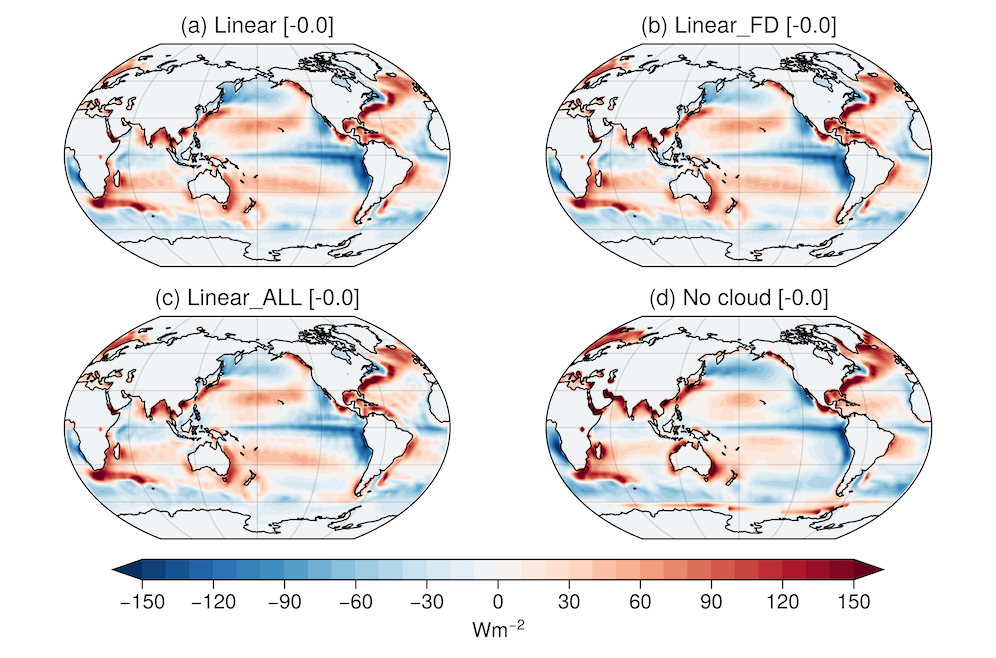
\includegraphics[width=1\linewidth]{{figs/change_of_CRE/Q-flux_cmp}.png}
% 	\caption[Comparison of spatial pattern of ocean heat transport (Q-flux).]{Annual mean Q-flux pattern (in W m$^{-2}$) derived from AMIP fixed-SST experiments with realistic continents and topography. The cloud schemes used are (a) linear, (b) linear\_FD and (c) linear\_ALL as in \tabref{tab:exps} and (d) no cloud scheme.}
% 	\label{fig:Q_flux_cmp}
% \end{figure}

% The AMIP fixed-SST experiments with linear cloud scheme described in \tabref{tab:exps} and a new fixed-SST simulation without clouds are used to derived the Q-flux, and the results are shown in \figref{fig:Q_flux_cmp}. The spatial patterns of Q-flux from different cloud schemes are similar, and have some differences from the simulation without cloud in subtropical and Southern Ocean regions. Q-flux can capture the ocean currents such as the Gulf Stream and cold tongue in the eastern tropical Pacific (\figref{fig:Q_flux_cmp}), and the positive value compensates for too little heating to the slab ocean by the surface flux from the `prescribed-SST’ run compared to the SST climatology. In this case, the Q-flux obtained from the run with the linear cloud scheme only is used in the following simulations. Also, the Q-flux remains the same in the control and perturbed experiments, but it is noted that the SST can change freely in response to different CO$_2$ forcing. 

\subsection{Perturbed parameter ensemble}
\label{sec:PPE_setup}
 
 As introduced in \secref{sec:cld_fbk_chap_intro}, the perturbed physics ensemble is a possible way to explore the sensitivity of GCM and examine the plausible spread of climate feedbacks. This method is adopted in this chapter to investigate the possible uncertainty of cloud feedbacks simulated from Isca with the simple cloud scheme from \chapref{ch:simple_cld_scheme}. In specific, a subset of parameters of the simple cloud scheme (see \tabref{tab:cld_scheme_summary}) are perturbed to get the members of PPE in Isca. There are many different options to vary the parameters to get the parameter space, but only one parameter is varied each time in our current perturbation. The perturbed parameters are listed in \tabref{tab:qflux_ppe_exps_summary}.
 
 \begin{table}[ht]
%\begin{sidewaystable}
	\caption{Design of the perturbed parameter experiments (PPEs). All simulations are run in T42 horizontal resolution.}
	\centering
	\renewcommand{\arraystretch}{1.5}
	\resizebox{\textwidth}{!}{
	\begin{tabular}{cc >{\raggedright}m{0.26\linewidth} m{0.6\linewidth}} 
	% control width, alignment for cells
	% https://texblog.org/2017/02/06/proper-tables-with-latex/
		\toprule
	    Index & Experiment & Parameter change & Description \\
		\midrule
		1 & Linear & Default values in \tabref{tab:cld_scheme_summary} & Simulations with Q-flux; Control (1$\times$CO$_2$) and perturbed (4$\times$CO$_2$) experiments \\
		2 & a\_surf & $a_{s}: 42 \rightarrow 20$ & Equivalent to decrease the critical relative humidity at the surface \\
		3 & a\_top & $a_{t}: 13 \rightarrow 10$ & Equivalent to decrease the critical relative humidity at the upper troposphere \\
		4 & Sc\_coeff\_c & $c: -0.1 \rightarrow -0.3$ & The added stratocumulus clouds should decrease \\
		5 & Sc\_coeff\_b & $b: 1.3 \rightarrow 1$ & The added stratocumulus clouds should decrease \\
		6 & Tmax &  $T_{max}:-5\rightarrow 0~^\circ$C & Increase the temperature threshold of the fraction of liquid cloud (Reff would increase) \\
		7 & Tmin & $T_{min}: -40\rightarrow -35~^\circ$C & Increase the temperature threshold of the fraction of ice cloud \\
		8 & Reff\_ice & $r_{e_ice}:25\rightarrow 50~\mu$m & Increase the default effective radius for ice cloud \\
		9 & Reff\_liq & $r_{e_ice}:14\rightarrow 12~\mu$m & Decrease the default effective radius for liquid cloud \\
		%rcl\_height &  & In-cloud liquid water mixing ratio is specified as a function of height, rather than as temperature \\
		10 & freezedry & On & Use the freezedry method \\
		11 & Sundqvist & On & Change the default cloud fraction scheme from linear to Sundqvist \\
		12 & cld\_water & $w_{l}=0.2$ & Increase the maximum of in-cloud water mixing ratio a box can reach \\
		%12 & qcl\_T & $q_{l}=0.2$ & In-cloud water mixing ratio as a function of height \\
		\bottomrule
	\end{tabular}
	}
	\label{tab:qflux_ppe_exps_summary}
%\end{sidewaystable}
\end{table}

The default parameters in \tabref{tab:cld_scheme_summary} are used for the control run (\textit{linear} in \tabref{tab:qflux_ppe_exps_summary}, but the freezedry adjustment introduced in \secref{sec:freezedry} is turned off. We do this for two reasons: First, the low-latitude regions usually contribute most to the spread of global mean cloud feedbacks, as suggested from previous studies and as to be shown later in \secref{sec:reg_contri_to_spread_of_cldfbk}, and the simulated cloud radiative effect in low and middle latitudes are fine without this adjustment. Therefore, keeping the schemes used in the study to its minimalism does not have large impact to the study of spread of cloud feedback. Second, the `freezedry' adjustment works well for the current climate (see \figref{fig:zonal_mean_cre}), but still needs some tests before it can be applied readily to the warming experiments. The perturbations for the cloud scheme alter either the cloud amount or cloud optical properties, as both are necessary components for radiation transfer calculation. Specifically, four experiments (i.e., \textit{a\_surf}, \textit{a\_top}, \textit{Sc\_coeff\_c}, \textit{Sc\_coeff\_b}) listed in \tabref{tab:qflux_ppe_exps_summary} are directly associated to the cloud amount, where \textit{a\_surf} and \textit{a\_top} adjust the cloud amount in large-scale cloud scheme (see \secref{sec:rh_cloud}), while \textit{Sc\_coeff\_c} and \textit{Sc\_coeff\_b} have impacts on the corresponding marine low cloud amount (see \secref{sec:marine_low_cld_scheme}). The perturbed parameter in \textit{Sundqvist} experiment is also related to possible changes in large-scale cloud amount. The other perturbed parameters or corresponding experiments are associated straightly with the optical properties of clouds, and these properties are altered by effective radius of cloud condensate (i.e., \textit{Reff\_ice} and \textit{Reff\_liq}), temperature thresholds for liquid or ice water fraction (i.e. \textit{Tmax} and \textit{Tmin}) or the maximum in-cloud water mixing ratio a box can reach (i.e. \textit{cld\_water}). Of course, these perturbations could have impact on cloud amount once the background condition evolves. The \textit{freezedry} experiment is also examined here for completeness, which can modify the behaviors of cloud scheme over high-latitude regions.

For each simulation with perturbed parameter, two runs are performed: one with CO$_2$ level similar to current climate (300 ppm; control run for each parameter), and the other with quadruple CO$_2$ (1200 ppm; perturbed run for each parameter). The control run is performed for 30 years, and as mentioned in \secref{sec:implementation_of_cosp}, the COSP is only active in the last 5 years. On the basis of the control run, the perturbed run is performed for another 30 years with CO$_2$ concentration quadrupled. Similarly, the satellite simulator is only enabled for the last 5 years in perturbed run. The spinup usually takes less than 20 years to finish in both runs. Other Isca setups, such as the convection scheme, large-scale condensation scheme and radiation scheme, are the same as those described in \secref{sec:exp_setup_and_dataset}. The only difference is that the simulations in \chapref{ch:simple_cld_scheme} are the AMIP-type fixed-SST experiments, while here the ocean heat flux (the `Q-flux') is prescribed. In the fixed-SST experiments, the changes in atmosphere could not feedback into the SST changes, and the Q-flux can make the simulation more realistic. Here we prescribe the derived `Q-flux' from a given distribution of SSTs \citep{Durack2018} following the method from \cite{Russell1985}, so that the SST can respond freely to the CO$_2$ forcing. The detailed description of how Q-flux is calculated can be found in \secref{sec:Q_flux_method}.

%\section{Results}
%\label{sec:results_cld_fbk}

\section{COSP evaluation}
\label{sec:eval_cosp}

\begin{figure}[ht]
    \centering
    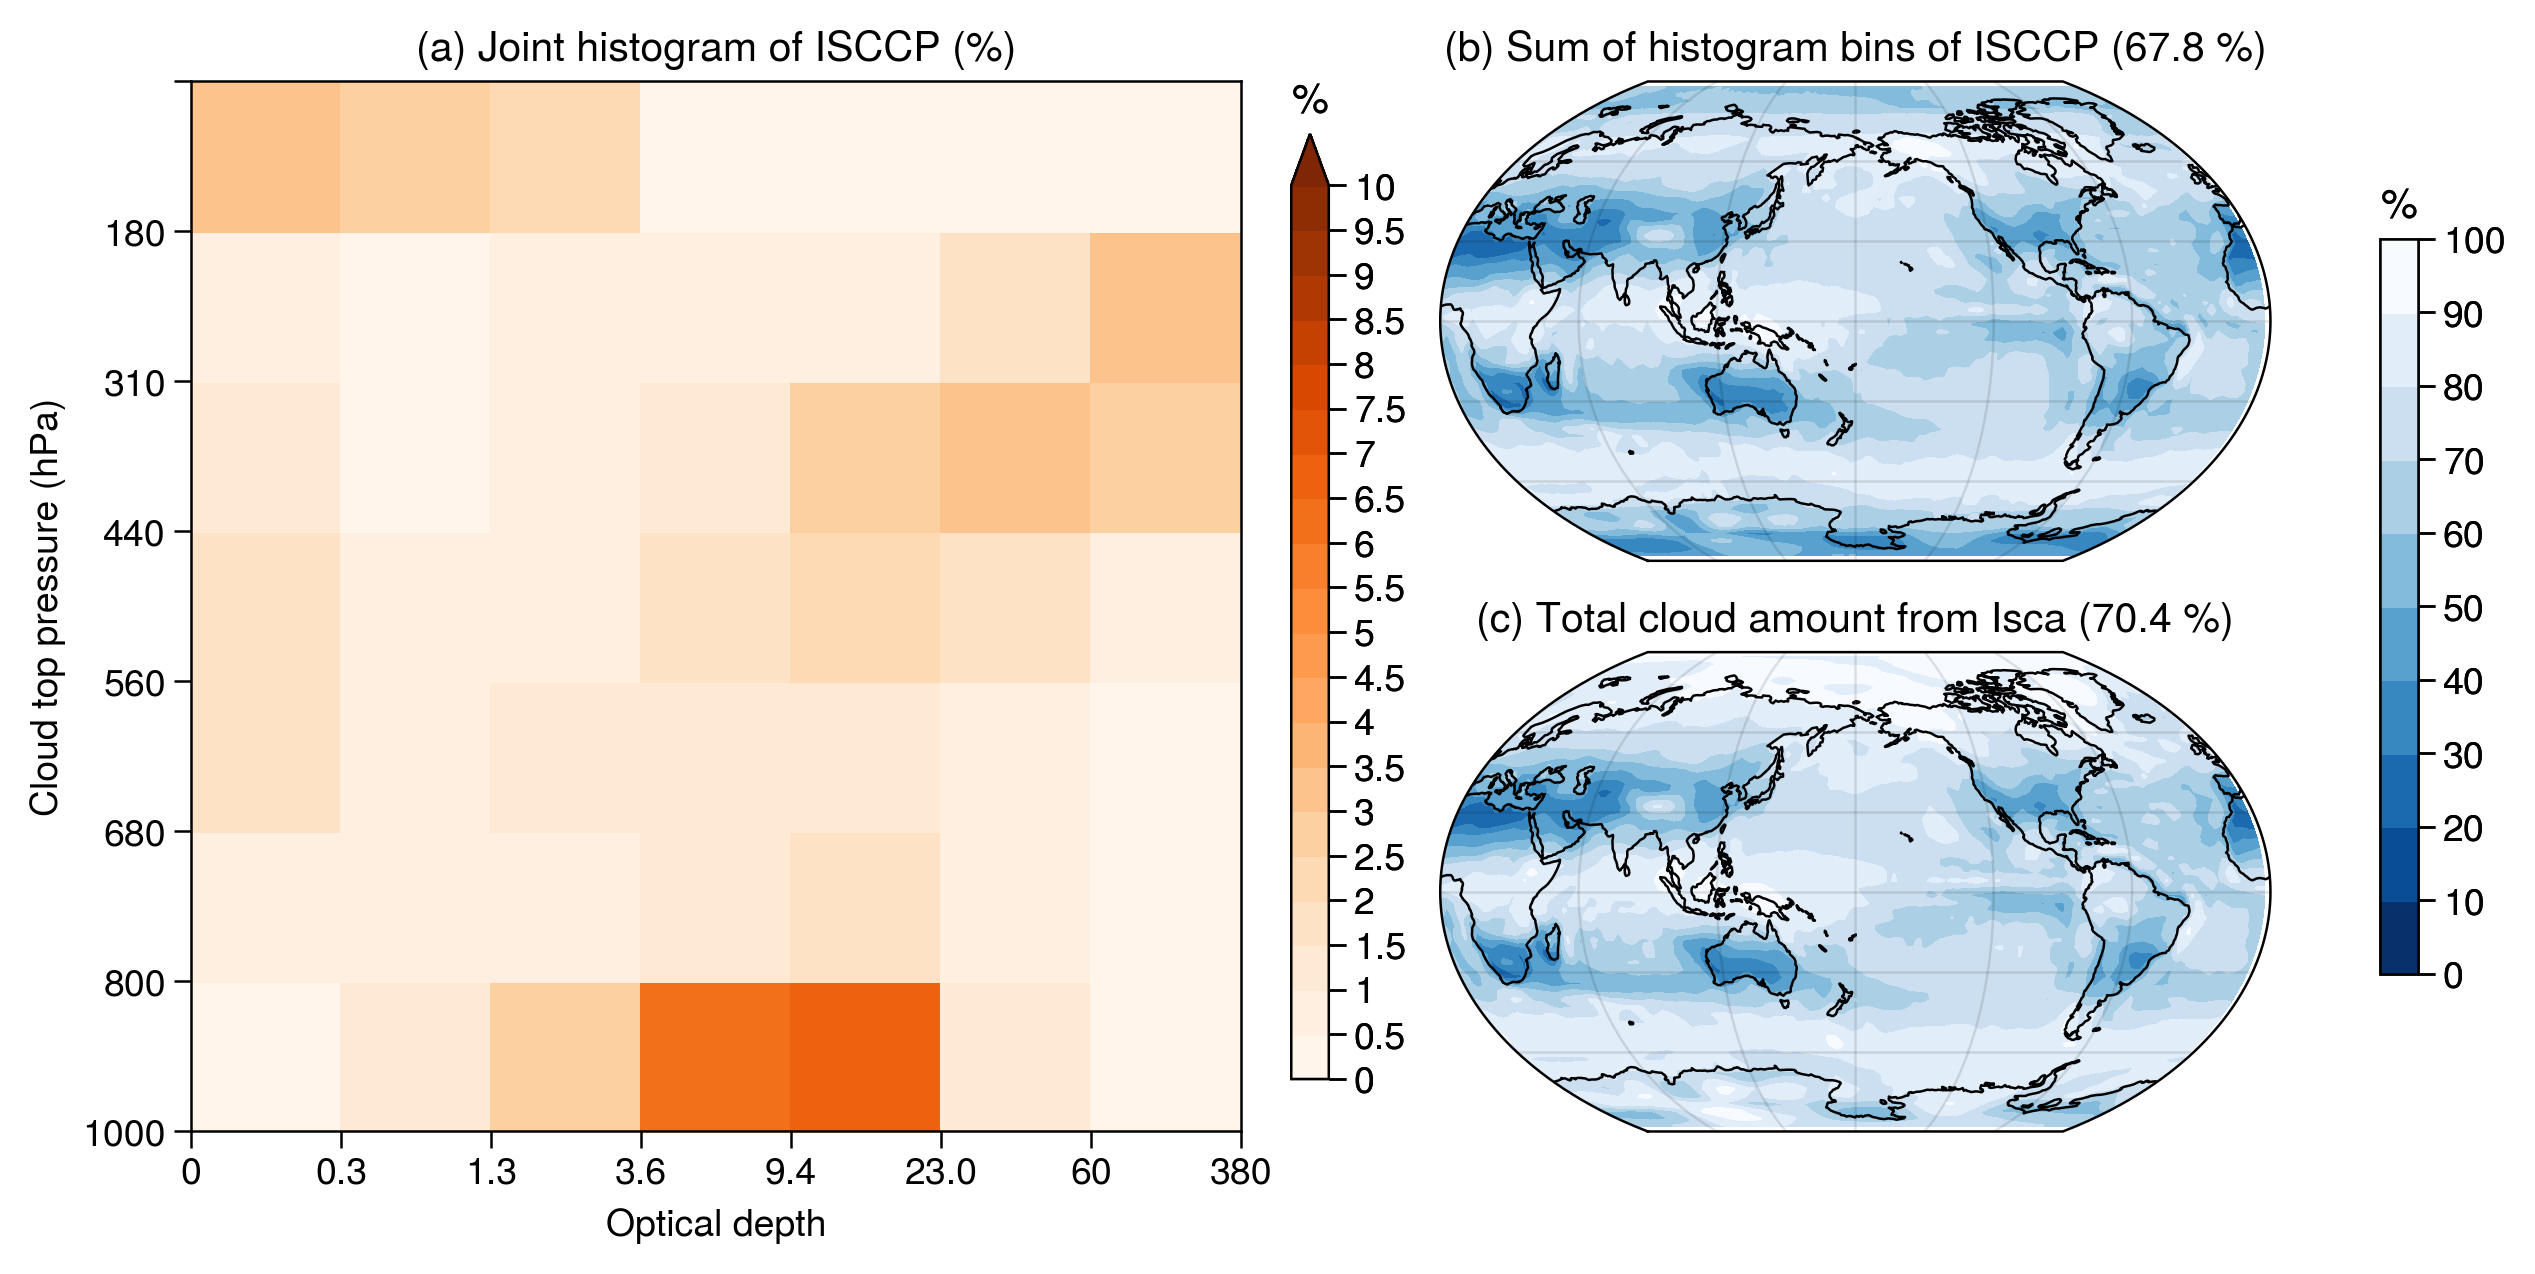
\includegraphics[width=1\linewidth]{{figs/change_of_CRE/cmp_isca_cosp_tot_cld_amt}.png}
    \caption{(a) The annual mean cloud fraction (\%) binned by the joint histogram of cloud top pressure and optical depth from ISCCP simulator implemented in Isca. (b) The sum of the histogram bins for each location from the ISCCP simulator of Isca. (c) The annual mean native total cloud amount from Isca simualtions based on max-random overlap assumption.}
    \label{fig:cmp_isca_and_sum_of_COSP}
\end{figure}

The implementation of COSP provides a new tool to compare Isca simulation results with the observations. For the Isca simulation with COSP, only ISCCP simulator \citep{Klein1999validation,Webb2001combining} is activated. One key output from ISCCP simulator is the joint histogram of cloud-top pressure and optical depth, as shown in \figref{fig:cmp_isca_and_sum_of_COSP}a, which bins the cloud fields into 7 CTP and 7 optical depth categories. The value in each bin represents the cloud fraction of that category. To make sure the COSP is correctly implemented in Isca, the diagnostics from COSP are compared to the Isca outputs. Specifically, following the method from \cite{Zelinka2012computing1} and \cite{Klein2013climate}, the sum of cloud cover over all bins of the joint histogram (\figref{fig:cmp_isca_and_sum_of_COSP} b) is compared with the diagnostic of total cloud cover (\figref{fig:cmp_isca_and_sum_of_COSP} c) from Isca that is computed without using the ISCCP simulator. It is noted that the global mean values of the two cloud covers are quite close, and the spatial patterns also match with each other, although we notice that some discrepancies appear over polar regions. This comparison suggests that the COSP is correctly implemented in Isca, and its output can be employed for the later analysis. 

\begin{figure}[ht]
    \centering
    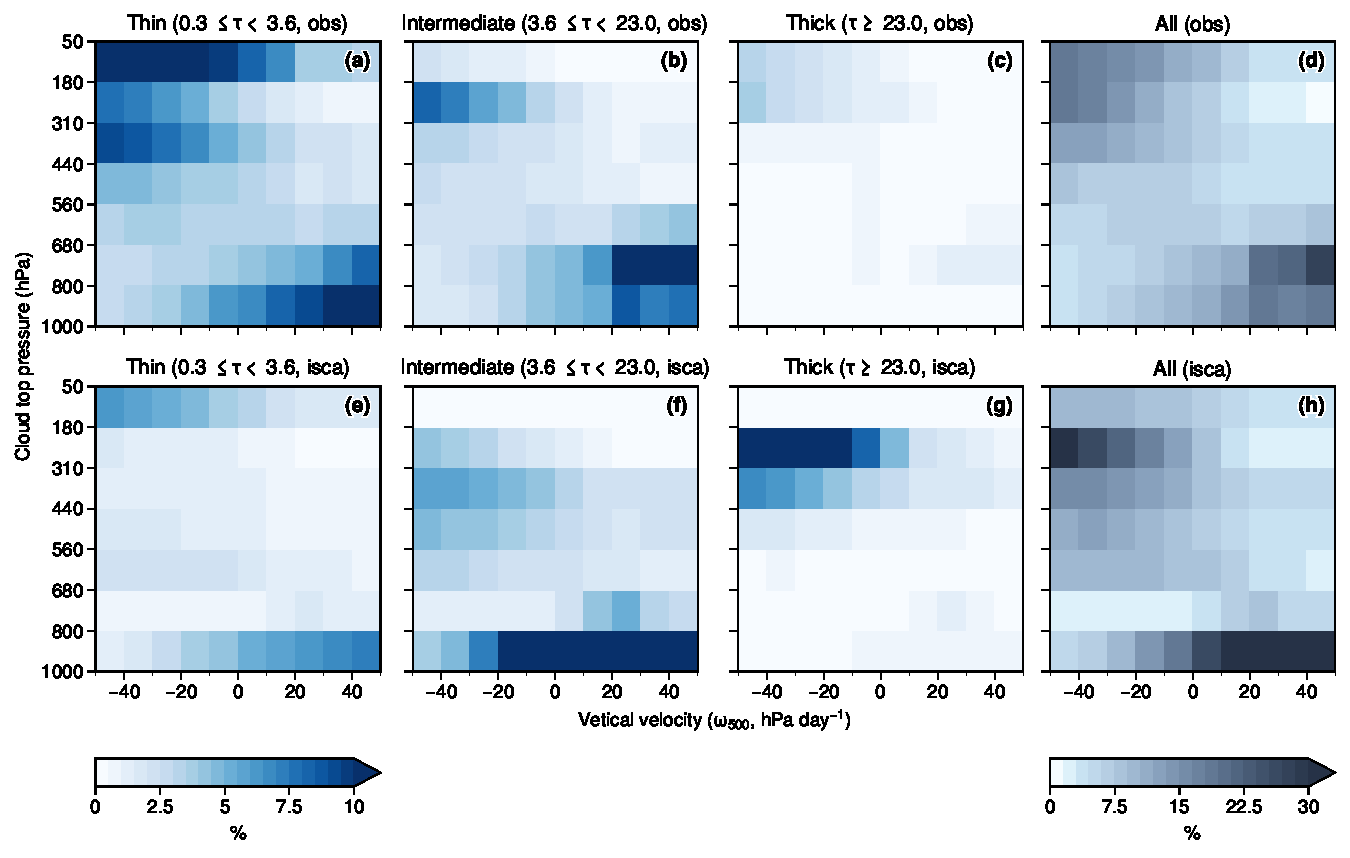
\includegraphics[width=1.0\linewidth]{{figs/change_of_CRE/clisccp_cloud_thickness_category_obs_isca_linear_sc}.pdf}
    \caption{Annual mean cloud frequency from (top row) GCM simulator-oriented ISCCP product (1998-2007) and (bottom row) one Isca simulation, sorted by vertical velocity at 500 hPa ($\omega_{500}$, units: hPa day$^{-1}$) and divided into different cloud thickness categories: (a, e) thin (0.3$\le\tau<$3.6), (b, f) intermediate (3.6$\le\tau<$23), (c, g) thick ($\tau\ge$23), and (d, h) all optical depths. For ISCCP, the $\omega_{500}$ is from ERA-Interim reanalysis (1998-2007). }
    \label{fig:tropical_clisccp_obs_isca}
\end{figure}

Here we also compared the ISCCP simulator outputs from Isca with observation directly. The Isca simulation is run with Q-flux with linear and low cloud scheme (shown in \tabref{tab:qflux_ppe_exps_summary}), while the observed cloud amount frequency distribution product is derived from the ISCCP D1 dataset \citep{Rossow1999advances} (available at \url{https://climserv.ipsl.polytechnique.fr/cfmip-obs/data/ISCCP}, last access: June 10, 2021), which is binned into six optical thickness categories, and each of these bins is further divided into seven cloud-top pressure groups. As shown in \figref{fig:tropical_clisccp_obs_isca}, 
the annual mean cloud frequency from  GCM simulator-oriented ISCCP product (covering the period from 1998 to 2007; top panels) and Isca simulation (bottom panels) is compared by sorting them into categories of different optical depth, namely thin (0.3$\le\tau<$3.6), intermediate (3.6$\le\tau<$23), thick ($\tau\ge$23), and and all optical depths. As this comparison is for tropical region (30$^\circ$S--30$^\circ$N) only, we further break down them into different dynamic regimes by vertical velocity at 500 hPa ($\omega_{500}$), similar to \cite{Wyant2006comparison} (see their Figs. 7--9). The observed ISCCP product is binned by $\omega_{500}$ from ERA-Interim reanalysis of the same period. In ISCCP observation product, the thin clouds (\figref{fig:tropical_clisccp_obs_isca}a) are a major contributor to the total cloud fraction (\figref{fig:tropical_clisccp_obs_isca}d) at all heights and all the dynamic regimes, especially near the surface over the subsidence regions and in upper troposphere over the ascent regimes. The intermediate clouds (\figref{fig:tropical_clisccp_obs_isca}b) are prevalent at the similar locations as the thin clouds, but the levels of maximum cloud fraction is different. The fraction of thick clouds (\figref{fig:tropical_clisccp_obs_isca}c) is the smallest among the three categories, and they are concentrated at the upper troposphere of ascending regions. Compared to the observation, the simulator diagnostics from Isca have have less thin clouds both in upper troposphere of upwelling region and in the lower troposphere of the subsidence regimes (\figref{fig:tropical_clisccp_obs_isca}e). With regard to the intermediate clouds, the Isca diagnostics have much similar pattern with observation, except the clouds concentrate near the bottom of CTP-bins over the subsidence regimes (\figref{fig:tropical_clisccp_obs_isca}f). The thick cloud fraction is overestimated in Isca at the ascent regimes near the tropopause (\figref{fig:tropical_clisccp_obs_isca}g). In total, Isca diagnostics have qualitatively similar CTP and optical depth histogram as observation (\figref{fig:tropical_clisccp_obs_isca}h), though the biases mentioned in the thin, intermediate and thick categories. These results suggest again that the COSP has run successfully in Isca.



\section{Simulated cloud feedbacks}
\label{sec:simu_cld_fbk}

One goal of this chapter is to investigate the underlying causes of the uncertainty in cloud feedbacks, but the first step is to evaluate the the cloud feedbacks from Isca simulations. Therefore, this section is arranged as follows: the simulated basic fields, such as temperature, relative humidity and cloud-related variables such as cloud fraction and cloud water content, and their possible changes under global warming in Isca simulations are examined in \secref{sec:basic_fields_ctrl_4xco2}, which could help us to understand the possible mechanisms of cloud feedback. The different diagnostics and methods that could be employed for the cloud feedback computation are compared in \secref{sec:cmp_cld_fbk_method_result} and from this section we will conclude that which method and diagnostic to be used for the future cloud feedback analysis. The spatial pattern and zonal mean structure of cloud feedbacks and their components are presented in \secref{sec:spatial_pattern_cld_fbk} and \secref{sec:zonal_mean_cld_fbk}, respectively.

\subsection{Basic fields}
\label{sec:basic_fields_ctrl_4xco2}

\begin{figure}[ht]
    \centering
    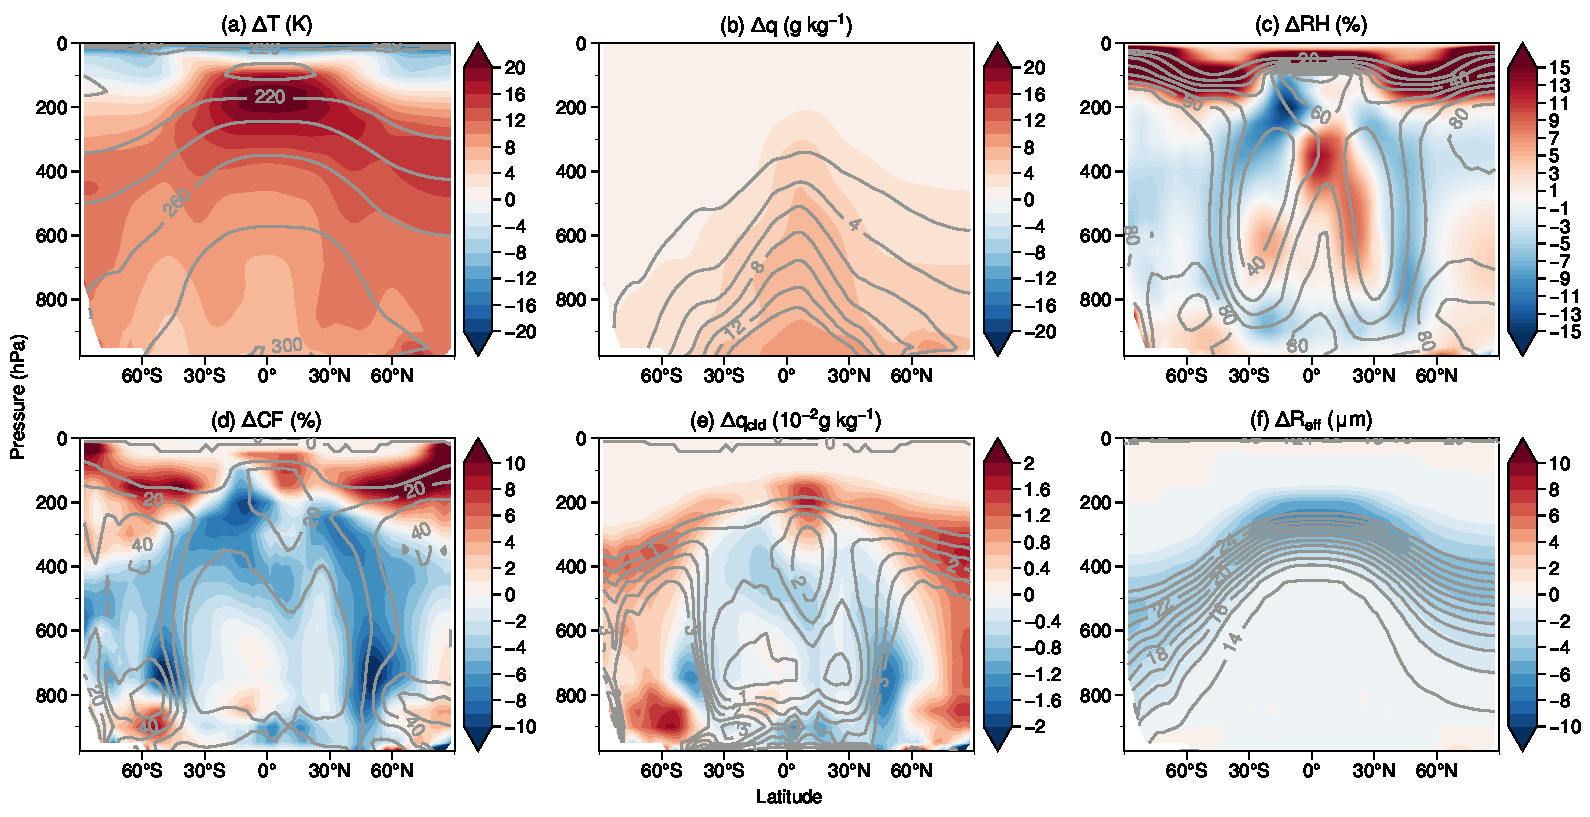
\includegraphics[width=1.0\linewidth]{{figs/change_of_CRE/zonal_mean_profile_change_basic_fields_ensemble_mean}.pdf}
    \caption{Zonal mean profiles (contour) for (a) temperature, (b) specific humidity, (c) relative humidity, (d) cloud fraction, (e) cloud water content and (f) effective radius and their responses (shading) to warming due to quadruple of CO$_2$ from Isca perturbed parameter ensemble.}
    \label{fig:zonal_mean_profile_change_ensemble_mean_for_cld}
\end{figure}

The mean and range of simulations of both present-day zonal mean profiles of some basic fields and their responses to global warming are exhibited in \figref{fig:zonal_mean_profile_change_ensemble_mean_for_cld}). Focusing on the cloud fraction (\figref{fig:zonal_mean_profile_change_ensemble_mean_for_cld}d), the ensemble mean results show an upward shift of clouds near the tropopause, and a decrease in clouds in most of the troposphere (cf. Fig. 5a of \citealt{Sherwood2020}). The changes in cloud fraction field basically reflect the changes in relative humidity (\figref{fig:zonal_mean_profile_change_ensemble_mean_for_cld}c) \citep[also see Fig. 2 of ][]{Sherwood2010}, although there are some discrepancies in tropical and subtropical regions. This is a problem of the relative humidity based cloud scheme, as it is possible that the relative humidity increases but the diagnosed cloud fraction decreases, if the increased relative humidity is still less than the threshold for the cloud formation \citep[e.g.,][]{Ming2018}. The fraction of liquid cloud fraction increases under global warming, so the effective radius, which is the weighted sum of liquid and ice cloud effective radii based on their each fraction, decreases accordingly (\figref{fig:zonal_mean_profile_change_ensemble_mean_for_cld}f).

% a poleward shift of clouds in midlatitudes, 

\begin{figure}[ht]
    \centering
    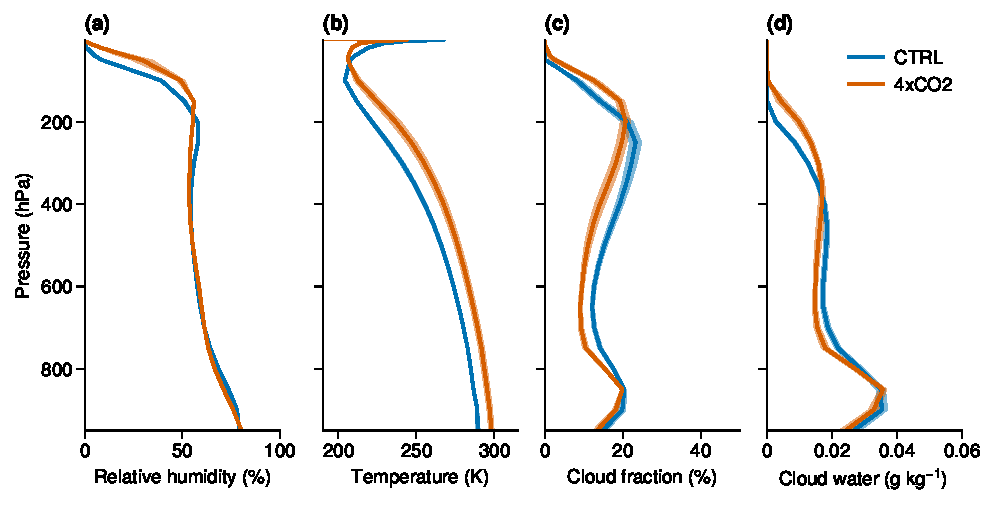
\includegraphics[width=1\linewidth]{{figs/change_of_CRE/global_multi_mean_profiles_for_PPE_full}.pdf}
    \caption{The ensemble and global mean profiles for (a) relative humidity, (b) temperature, (c) cloud fraction and (d) cloud water content in control (1$\times$CO$_2$) and global warming (4$\times$CO$_2$) experiments in Isca perturbed parameter ensemble.}
    \label{fig:global_mean_profiles_from_ctrl_4xco2}
\end{figure}

To have a clear look at the changes of the simulated fields under global warming in Isca simulations, the ensemble and global mean profiles from the PPE are shown in \figref{fig:global_mean_profiles_from_ctrl_4xco2}. There is a clear reduction of cloud fraction in lower and middle tropospheres and a upward shift of cloud fraction at upper troposphere in the global warming experiment of Isca (\figref{fig:global_mean_profiles_from_ctrl_4xco2}c). The latter change can be inferred from the relative humidity changes under global warming (\figref{fig:global_mean_profiles_from_ctrl_4xco2}a), but we also notice that there are some discrepancies in middle troposphere between the relative humidity and cloud fraction fields, as shown in \figref{fig:zonal_mean_profile_change_ensemble_mean_for_cld}. The cloud water content changes under global warming in \figref{fig:global_mean_profiles_from_ctrl_4xco2}d follow the changes in cloud fraction field. All these changes could assist us in understanding the changes in cloud radiative effect under global warming (i.e., cloud feedback) in \secref{sec:spatial_pattern_cld_fbk}.

% \begin{figure}[ht]
%     \centering
%     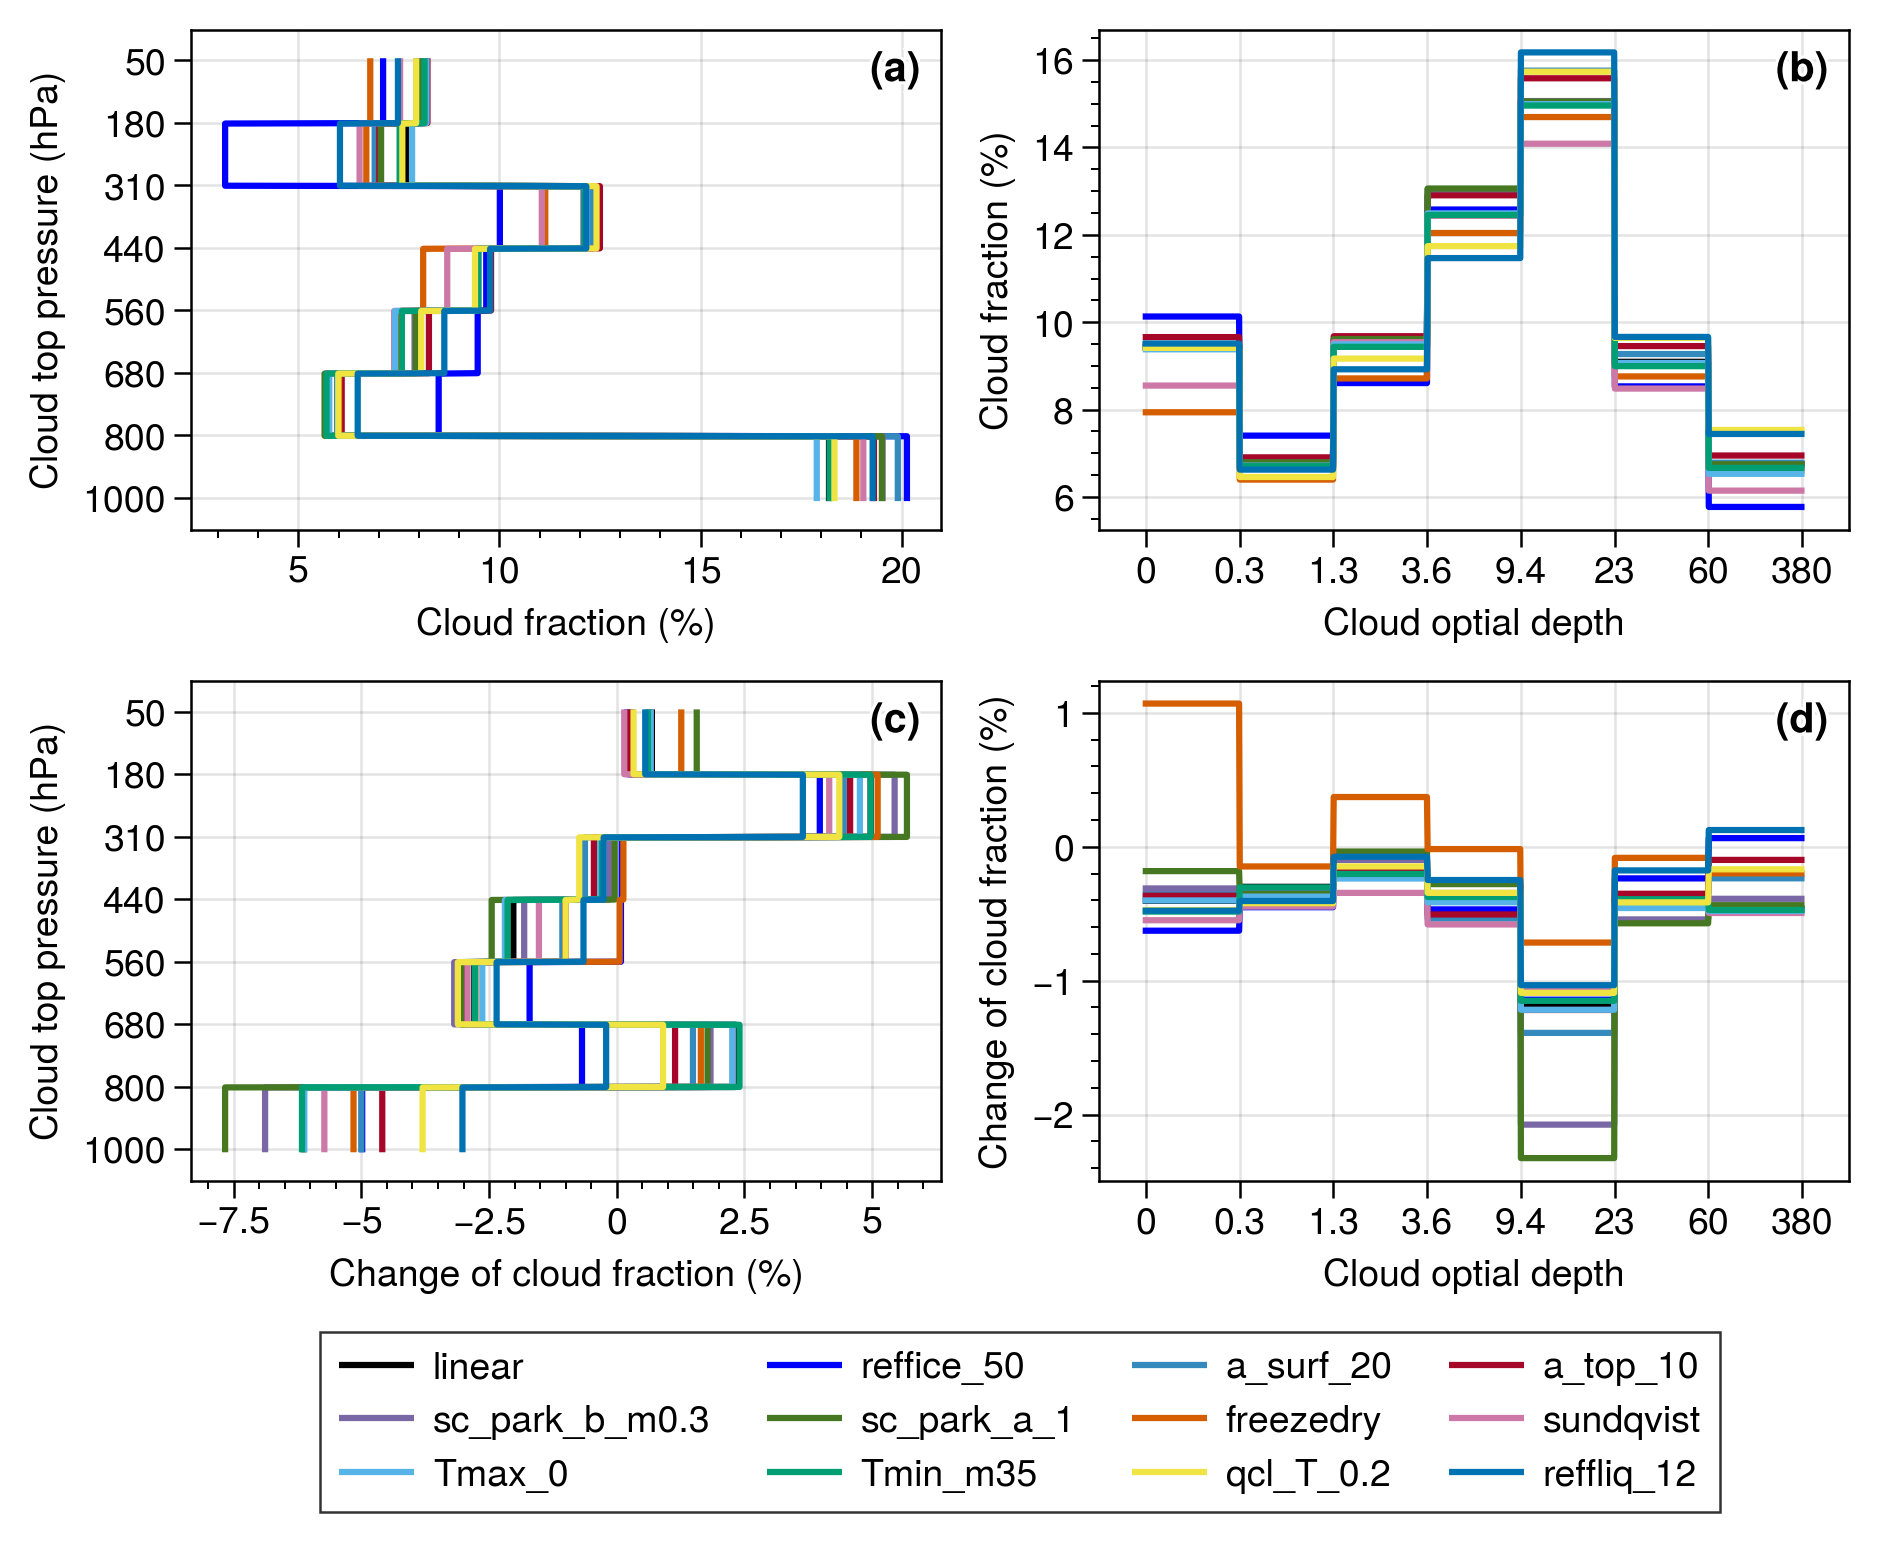
\includegraphics[width=1.0\linewidth]{{figs/change_of_CRE/change_of_cld_fraction_view_from_clisccp}.png}
%     \caption{The cloud fraction changes for different optical depth categories.}
%     \label{fig:change_of_cld_from_isccp_perspective}
% \end{figure}

\subsection{Comparison of cloud feedback calculation}
\label{sec:cmp_cld_fbk_method_result}

One goal of this chapter is to evaluate the cloud feedabcks from Isca simulations. The methods used in previous studies to estimate cloud feedback are introduced in \secref{sec:method_cloud_fbk}, including the estimation from cloud radiative effect (CRE; i.e. the all-sky minus clear-sky downward radiative flux at TOA) and the partial radiative perturbation (or PRP) methods. An alternative to the PRP method is the kernel method, which is more efficient than the PRP method, and can be widely used among different models \citep{Soden2006,Soden2008}. The traditional radiative kernel method can account for the masking effect of clouds via the difference between the all-sky and clear-sky kernels when calculating the cloud feedback, but it is hard to decompose the bulk cloud feedback into different components. The cloud kernel method proposed by \cite{Zelinka2012computing1,Zelinka2012computing2} calculates the cloud feedback in the space of the ISCCP joint histogram of CTP and cloud optical depth, which facilitates the diagnosis of cloud changes consistently across the different models and can track the cloud feedback to the changes in cloud altitude, amount or optical thickness, and thus to different cloud types \citep{Siebesma2020clouds}. 

Here we compute and compare the cloud feedback from Isca simulations with various diagnostics and methods. As summarized by \cite{Zelinka2013} (see their Table 1), based on the CRE or the kernel derived cloud-induced radiation anomalies diagnostics, there still two ways using them to estimate the cloud feedback. One is to calculate the cloud feedback by normalizing the CRE or cloud-induced radiation anomalies by the change of surface temperature between perturbed and control simulations; The other is to use the Gregory method \citep{Gregory2004}, which regresses the time series of radiation anomalies against the surface temperature changes and the slope is the feedback we wanted. The advantage of the Gregory method is that it accounts for the rapid adjustments, which is usually considered as part of radiative forcing \citep{Andrews2012cloud,Siebesma2020clouds}. In addition, the CRE based diagnostic is affected by the cloud masking effect, while the cloud-induced radiation anomalies derived from cloud radiative kernel method is not affected by the masking effect \citep{Zelinka2013}.

\figref{fig:gregory_plot_for_CRE_and_kernel_flux} shows the Gregory plot of the global and annual mean anomalies in cloud-induced TOA radiative flux against the change in global mean surface temperature ($\Delta T_s$). These flux anomalies are estimated from CRE and cloud radiative kernel respectively, so they are corresponding to II and IV categories in \tabref{tab:four_methods_cldfbk_results}. The cloud-induced radiative flux anomalies at TOA ($\Delta R_c$) is computed as follows:
\begin{equation}
    \Delta R_{C}=\sum_{p=1}^{7} \sum_{\tau=1}^{7}\left(K_{p \tau} \Delta C_{p \tau}\right),
\end{equation}
where $K_{p\tau}$ is the cloud radiative kernel at each CTP-optical depth bin of ISCCP histogram, in which both the CTP and optical depth ($\tau$) categories have 7 bins. In this calculation, the cloud radiative kernels are multiplied by changes in ISCCP simulator-diagnosed cloud fraction $\Delta C_{p\tau}$ between a perturbed and control climate and summed over all CTP and optical depth categories. It is clear that there is a sign change in the slope of longwave cloud feedback (\figref{fig:gregory_plot_for_CRE_and_kernel_flux}a), where the slope changed from -0.31 Wm$^{-2}$K$^{-1}$ in category II (CRE + Gregory) to 0.35 Wm$^{-2}$K$^{-1}$ in category IV (kernel + Gregory). The longwave forcing term in category II is more negative than that in category IV due to the cloud masking effect. For example, \cite{Andrews2012cloud} found that the instantaneous cloud masking effect for longwave CRE is about -0.62 Wm$^{-2}$ in response to doubling CO$_2$ (see their Table 2). Similarly, \cite{Soden2004} got a better estimation of cloud longwave feedback by assuming the cloud-masking effect is uniform and about 0.69 Wm$^{-2}$.

\begin{figure}[ht]
    \centering
    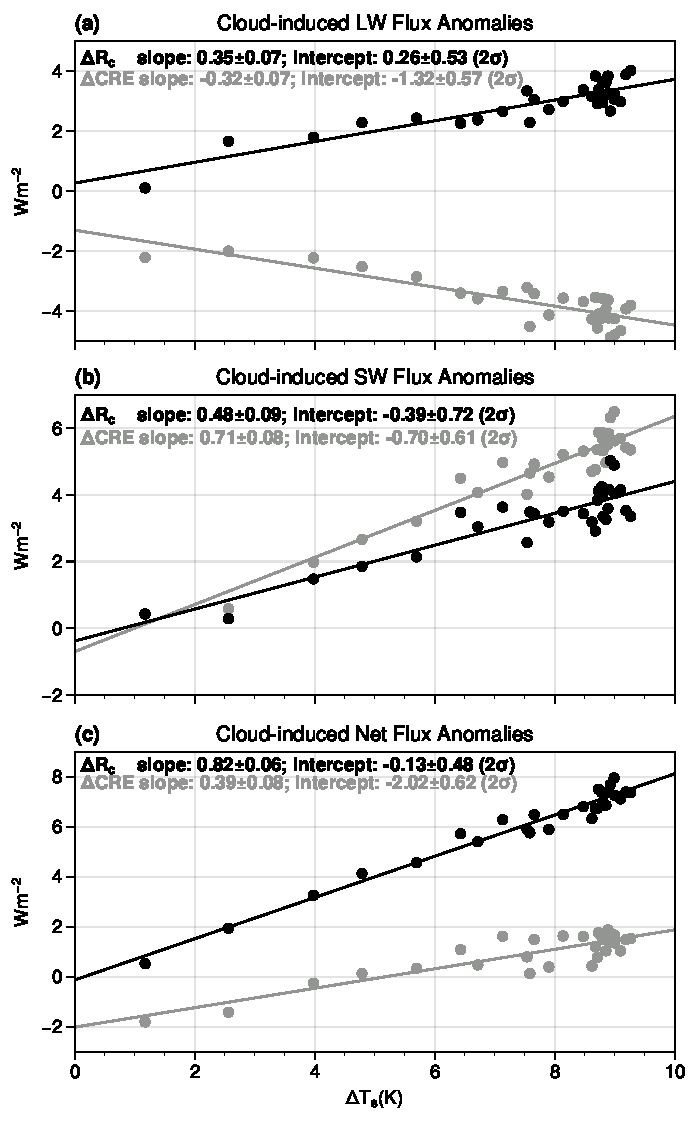
\includegraphics[width=0.6\linewidth]{{figs/change_of_CRE/gregory_plot_all_cld_fbk_v2}.pdf}
    \caption{Global and annual mean anomalies in cloud-induced TOA (a) longwave (LW), (b) shortwave (SW) and (c) net radiative flux against global mean surface temperature change ($\Delta T_s$). The black dots and lines are fluxes derived from cloud radiative kernel method \citep{Zelinka2012computing1}, while the gray ones are for the cloud radiative effect (CRE).}
    \label{fig:gregory_plot_for_CRE_and_kernel_flux}
\end{figure}

\begin{table}[ht]
    %\begin{sidewaystable}
	\caption{Comparison of longwave (LW), shortwave (SW) and net cloud feedbacks estimated from different methods and diagnostics as summarized in Table 1 (categories I--IV) of \cite{Zelinka2013} (units: Wm$^{-2}$K$^{-1}$).}
	\vspace{0.5em}
	\centering
	\renewcommand{\arraystretch}{1.2}
	\resizebox{1.0\textwidth}{!}{
	\begin{tabular}{>{\centering}m{0.4\linewidth} ccc ccc} 
	    % control width, alignment for cells
	    % https://texblog.org/2017/02/06/proper-tables-with-latex/
		\toprule
		\multirow{2}{*}{Diagnostic} & \multicolumn{3}{c}{$\Delta R/\Delta T_s$} & \multicolumn{3}{c}{\thead{Slope of $\Delta R$ against $\Delta T_s$ \\(Gregory method)}}\\
		\cline{2-4}\cline{5-7}
		 & LW & SW & Net & LW & SW & Net \\
		\midrule
		%CRE anomalies & & & & & & \\
		%Kernel-derived cloud-induced radiation anomalies & & & & & & \\
		CRE anomalies   &  -0.475 &   0.626 &    0.150 (I) &    -0.317 &     0.706 &      0.389 (II) \\  
        Kernel-derived cloud-induced radiation anomalies &   0.365 &   0.440 &    0.805 (III) &     0.346 &     0.479 &      0.825 (IV)\\  
        \bottomrule
	\end{tabular}
	}
	\label{tab:four_methods_cldfbk_results}
    %\end{sidewaystable}
\end{table}

The cloud feedback is also calculated by the change of CRE directly, as shown in the categories I and III in \tabref{tab:four_methods_cldfbk_results}. Focusing on the second row (the radiative kernel based diagnostic), we can find that the cloud feedback parameters from the categories III and IV are much similar, indicating that neglecting the rapid cloud adjustments has relative small impact on cloud feedback when using the kernel-based diagnostic. In contrast, comparing to the results in first and second rows of \tabref{tab:four_methods_cldfbk_results}, we can find the cloud masking effect do have a large impact on the cloud feedback calculation, especially for the longwave cloud feedbacks. For instance, the sign of longwave cloud feedback parameter changed when using  kernel-derived diagnostic rather than CRE related diagnostic in \tabref{tab:four_methods_cldfbk_results} (category I to III or II to IV).

%  This is also true for CRE based diagnostic (the first row in \tabref{tab:four_methods_cldfbk_results}). For example, the cloud feedback has relative small changes from category I to category II in Table 1 of \cite{Zelinka2013}

% The spatial pattern comparison?

In summary, from this comparison we conclude that the CRE based diagnostics can be impacted by the cloud masking effect, especially for the longwave components; while the kernel-derived diagnostics are nearly not impacted by the masking effect. Also, comparing to the $\Delta R/\Delta T_s$ method with the Gregory method, we find the rapid adjustment has little influence on the feedback calculation when using kernel-based diagnostics. As the COSP needs to be active from the start of the simulation when employing the Gregory method, it is time consumptive if all the simulations in PPE use this method. Therefore we adopt the kernel-derived diagnostics but estimate the cloud feedback from $\Delta R/\Delta T_s$ in current study.

\subsection{Spatial pattern}
\label{sec:spatial_pattern_cld_fbk}

\begin{figure}[ht]
    \centering
    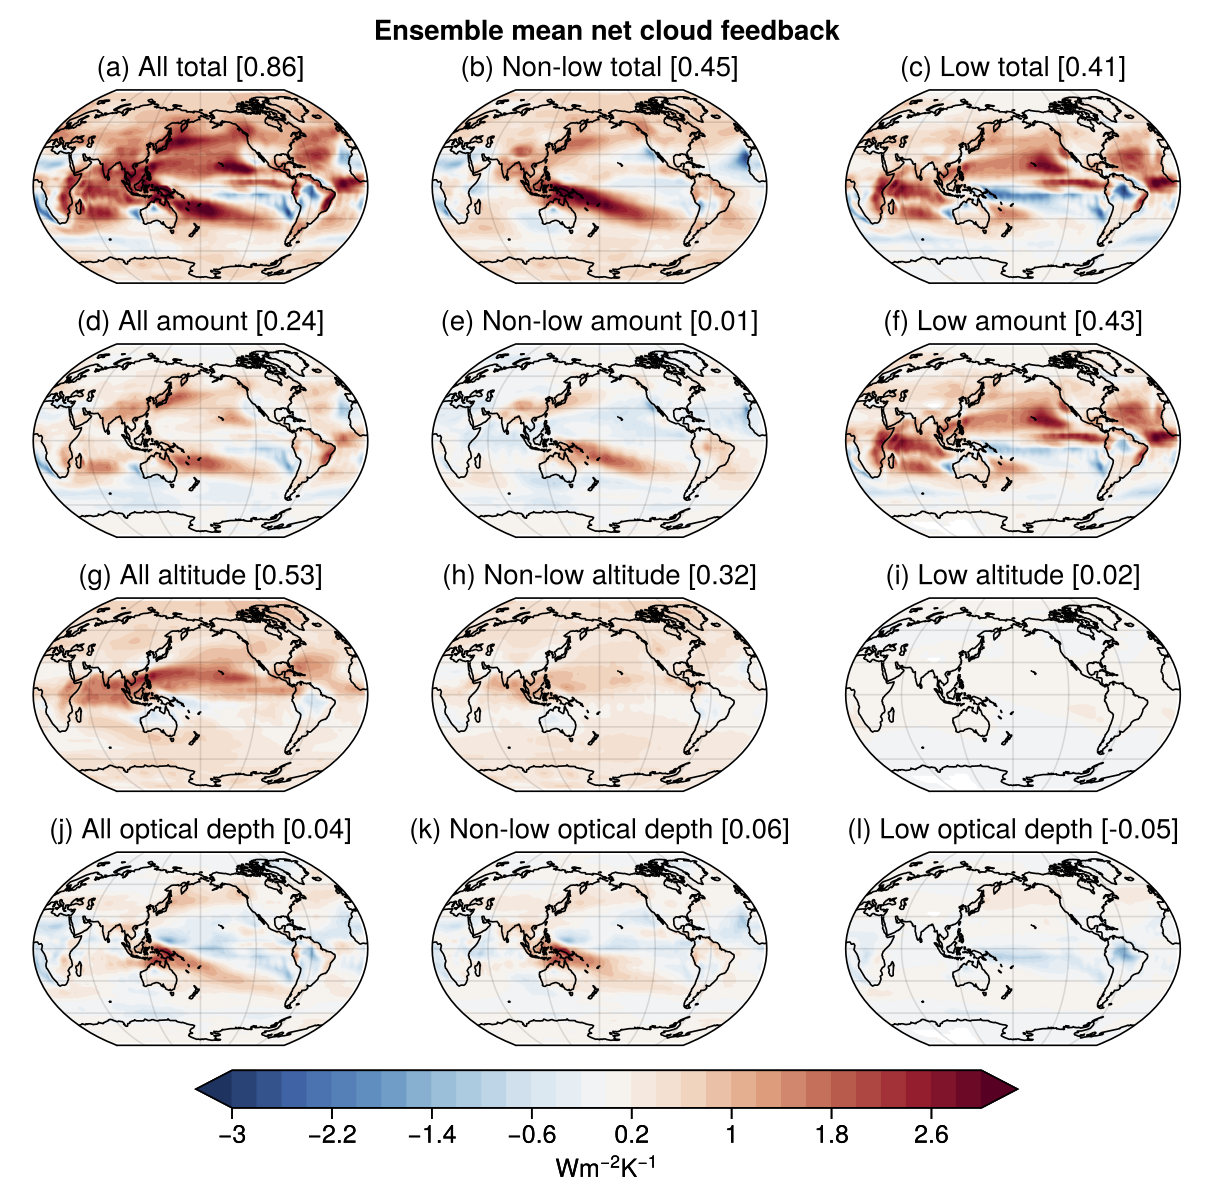
\includegraphics[width=0.9\linewidth]{{figs/change_of_CRE/annual_mean_net_cld_fbk_map}.png}
    \caption{The ensemble and annual mean net cloud feedback and its amount, altitude, and optical depth components from Isca perturbed paramerter ensemble for all clouds (left), non-low clouds (cloud top pressure, CTP ≤ 680 hPa; middle), and only low clouds (CTP > 680 hPa; right). Global mean values (in Wm$^{-2}$K$^{-1}$) are shown in brackets in the title of each panel.}
    \label{fig:net_cld_fbk_components_map}
\end{figure}

The comparisons in \secref{sec:cmp_cld_fbk_method_result} have shown that the cloud radiative kernel based diagnostics and the $\Delta R/\Delta T_s$ method can provide a relative accurate calculation of cloud feedback, and thus in this section all the feedbacks are calculated in this way. Another advantage of using this method is that it can break down the total cloud feedback into various components according to cloud altitude and types. The ensemble and annual mean spatial pattern of the cloud feedbacks from the Isca PPE are displayed in \figref{fig:net_cld_fbk_components_map}.

The net cloud feedback simulated in Isca is positive in most locations ( \figref{fig:net_cld_fbk_components_map}a), and the global mean quantity is about 0.86 Wm$^{-2}$K$^{-1}$, a value larger than the multi-model ensemble mean ($\sim$ 0.5 Wm$^{-2}$K$^{-1}$) but still within the range of net cloud feedbacks among all the CMIP5/6 models (see Fig. 1 of \citealt{Zelinka2020causes}). The decomposition of the net cloud feedback based on cloud radiative kernel method could provide some insights to understand the cloud feedbacks. In \figref{fig:net_cld_fbk_components_map}, the total cloud feedback is broken down into amount (second row), altitude (third row) and optical depth (fourth row) ingredients, repeated for all (left column), non-low (CTP$\le$680 hPa; middle column) and low (CTP>680hPa; right column) clouds, respectively. In terms of the cloud amount feedback, the global mean low cloud component is strongly positive (\figref{fig:net_cld_fbk_components_map}f), while the non-low component is close to zero (\figref{fig:net_cld_fbk_components_map}e). The positive low cloud amount feedback is probably due to the reduction of cloud amount in lower troposphere, as shown in \figsref{fig:zonal_mean_profile_change_ensemble_mean_for_cld}d and  \ref{fig:global_mean_profiles_from_ctrl_4xco2}c. The low cloud amount feedback is strongly positive over Northern Pacific and equatorial Eastern Pacific regions. However, the ensemble mean low cloud amount feedback in Isca PPE is negative in subtropical east Pacific regions off the west coast of Peru, which is due to the increase of low cloud amount in these regions under global warming (not shown here) and is not consistent with the positive low cloud amount feedback over these locations in CFMIP models (see the Fig. 2 of \citealt{Zelinka2016insights}). One plausible explanation for this is that the low cloud scheme (see \secref{sec:marine_low_cld_scheme}) depends too strongly on the inversion strength, thereby inducing more low clouds under global warming (to be discussed in Sec. xxxx about cloud controlling factor analysis). The other  low cloud feedback components such as altitude (\figref{fig:net_cld_fbk_components_map}i) and optical depth (\figref{fig:net_cld_fbk_components_map}l) feedbacks are quite weak globally. Regarding to the non-low cloud amount, the altitude feedback is positive universally (\figref{fig:net_cld_fbk_components_map}h), with the global mean value being 0.32 Wm$^{-2}$K$^{-1}$. This is associated to the upward shift the free tropospheric clouds under global warming (\figref{fig:global_mean_profiles_from_ctrl_4xco2}c), and could be explained by the fixed anvil temperature assumption \citep[e.g.,][]{Hartmann2002FAT, Ceppi2017}. Under this assumption, the CTP temperature does not warming in step with the surface warming, implying that more longwave radiation is trapped in the atmosphere. The global mean value of other components of non-low cloud feedbacks are not evident as the altitude feedback, as indicated in \figsref{fig:net_cld_fbk_components_map}e and \ref{fig:net_cld_fbk_components_map}k. One plausible reason is that the longwave and shortwave radiative effects of high clouds nearly cancel with each other \citep{Kiehl1994observed}, so the change of non-low cloud amount leads to a near-zero net amount feedback (also see \figref{fig:global_mean_cld_fbk_scatter}b). Similarly, as pointed by \cite{Zelinka2016insights}, the increase in optical depth for non-low clouds would induce the reduction of incoming solar radiation and outgoing longwave radiation due to the increase of cloud albedo and emissivity, respectively, so the offset results in near-zero global mean optical depth feedback for non-low clouds.

% As we know, the cloud feedback can arise from changes in different cloud properties such as cloud amount, location and optical thickness, as well as the coupling between clouds and circulation \citep[see Fig. 7.11 in ][]{Stocker2013}. 
%\citep[e.g.][]{Zelinka2017}.
%The partition of cloud feedbacks into different components

In fact, compared to the cloud feedback in CFMIP1/2 models (see their Fig. 2 of \citealt{Zelinka2016insights}), the feature of strong negative cloud feedback in extra-tropics, particular over the Southern Ocean, is missing Isca simulations (\figref{fig:net_cld_fbk_components_map}a). This negative feedback in CFMIP models is from the negative optical depth feedback, which likely arises from two reasons: The first is that the adiabatic cloud water content increases with temperature, and increases more strongly at lower temperature \citep{Betts1987thermodynamic}; The second is the phase change in mixed-phase clouds under global warming, as there are more liquid condensate that usually have smaller particle size, reduced precipitation efficiency and longer life time than ice clouds \citep{Ceppi2017}. However, this is not well represented in the simple cloud scheme due to lack of microphysical processes and the direct interaction between cloud and convection schemes.

%In summary, the simulated spatial patterns of cloud feedbacks in the Isca PPE 

\subsection{Zonal mean structure}
\label{sec:zonal_mean_cld_fbk}

\begin{figure}[ht]
    \centering
    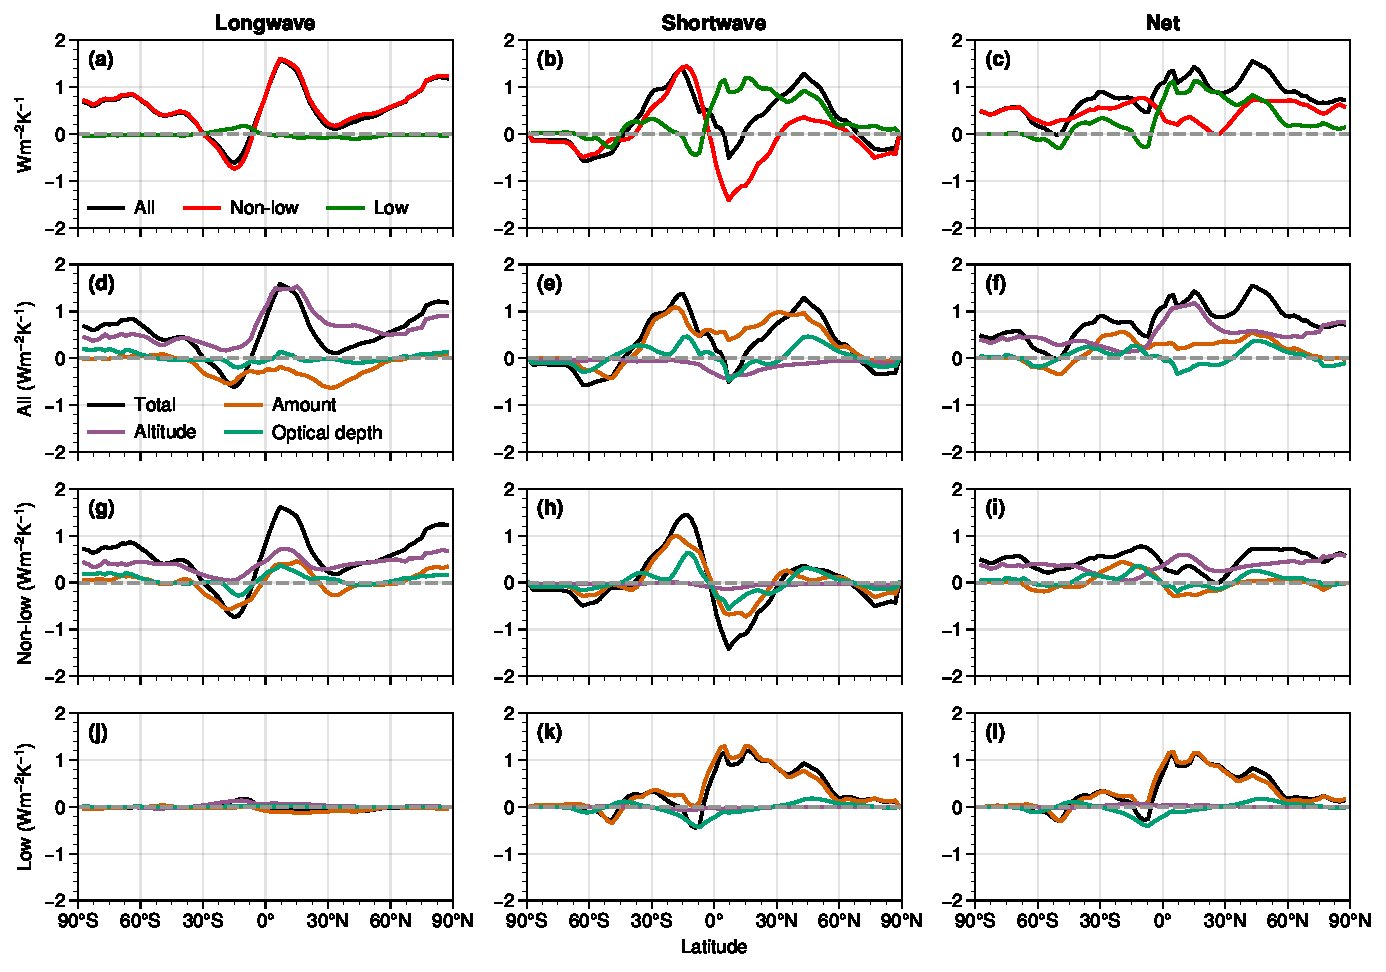
\includegraphics[width=1.0\linewidth]{{figs/change_of_CRE/annual_and_zonal_mean_cld_fbk}.pdf}
    \caption{Zonal and ensemble mean (left column) longwave, (middle column) shortwave, and (right column) net cloud feedbacks from Isca perturbed parameter ensemble. (a-c) Total cloud feedbacks and their separate contributions from non-low (red) and low (green) clouds. Total cloud feedbacks (black) and their amount (orange), altitude (purple), and optical depth (green) components for (d-f) all clouds, (g-i) non-low clouds only, and (j-l) low clouds only.}
    \label{fig:zonal_mean_cld_fbk_ensemble}
\end{figure}

The ensemble and zonal mean longwave, shortwave and net cloud feedbacks from the PPE of Isca are displayed in \figref{fig:zonal_mean_cld_fbk_ensemble}. If the total cloud feedback is decomposed into non-low (above 680 hPa) and low (below 680 hPa) components, it is evident that the non-low clouds dominate the zonal mean structure of longwave feedback (\figref{fig:zonal_mean_cld_fbk_ensemble}a), while the low cloud component is quite close to zero. This is reasonable as the temperature difference between low clouds and Earth surface is small compared to that of high clouds, so the longwave feedback is not significant (\figref{fig:zonal_mean_cld_fbk_ensemble}j). The longwave feedback of high clouds in fact is dominated by its altitude component, as shown in \figsref{fig:zonal_mean_cld_fbk_ensemble}d and \ref{fig:zonal_mean_cld_fbk_ensemble}g. As discussed in \secref{sec:spatial_pattern_cld_fbk}, this could be explained by the fixed-anvil temperature assumption \citep{Hartmann2002FAT}. In terms of the shortwave cloud feedback (middle column of \figref{fig:zonal_mean_cld_fbk_ensemble}), both low and non-low clouds have large impact on the zonal structure of cloud feedback (\figref{fig:zonal_mean_cld_fbk_ensemble}b). 

For shortwave cloud feedback, in the tropical and subtropical region, the low cloud feedback is usually positive, possibly due to the reduction of low cloud amount, as indicated by the positive low cloud amount feedback in \figref{fig:zonal_mean_cld_fbk_ensemble}k. The non-low cloud feedback (\figref{fig:zonal_mean_cld_fbk_ensemble}h) from Isca simulation shows the asymmetry pattern in subtropical regions, in which the positive feedbacks in 0-40$^\circ$S and 30$^\circ$-60$^\circ$N are due to the reduction of high cloud amount  and negative feedback in 0-30$^\circ$N is due to the increase in high cloud amount. 

The net cloud feedabck (right column of \figref{fig:zonal_mean_cld_fbk_ensemble}) is the sum of longwave and shortwave components. For the low clouds, the positive cloud feedback in tropical and subtropical regions are dominated by cloud amount changes (\figref{fig:zonal_mean_cld_fbk_ensemble}l), but there is no clear negative optical depth feedback in midlatitudes, which disagrees with the CMIP models (see Fig. 5 of \citealt{Sherwood2020} and Fig. S7 of \citealt{Zelinka2016insights}). This missing feature in Isca simulations arises from its absent representation of microphysical processes of mixed-phase clouds over those regions. For the middle and high clouds, the overall positive feedabck among all the latitudes is major from the altitude feedback (\figref{fig:zonal_mean_cld_fbk_ensemble}i). In sum, the positive low cloud amount feedback and high cloud altitude feedback are two basic features that account for the positive cloud feedback in Isca simulations (\figsref{fig:zonal_mean_cld_fbk_ensemble}c and \ref{fig:zonal_mean_cld_fbk_ensemble}f).

% % The upward shift of the high clouds keeps their cloud top temperature relatively unchanged under the fixed-anvil temperature assumption \citep{Hartmann2002FAT}, meaning that the high clouds do not warm in step with the surface warming.

\section{Spread of cloud feedback}
\label{sec:spread_of_cld_fbk_in_PPE}

\secref{sec:simu_cld_fbk} has introduced the simulated cloud feedback from Isca simulations. In this section, the spread of simulated cloud feedback is to be investigated. As introduced in \secref{sec:simu_cld_fbk}, the simulated cloud feedback is decomposed physically into cloud amount, altitude and optical depth components through the cloud radiative kernel method \citep{Zelinka2012computing1,Zelinka2012computing2}. Also, this method can be performed separately for the decomposition of low (CTP > 680 hPa) and non-low (CTP < 680 hPa) clouds, which considers the probability that the boundary layer clouds may behave differently from the clouds in free troposphere and can make the analysis of the change in free-tropospheric clouds more coherently \citep{Zelinka2016insights}. As suggested by \cite{Zelinka2016insights}, this refined decomposition can provide some insights for us to understand the underlying causes of spread in cloud feedback. Here we employ the cloud radiative kernel method to repeat the decomposition for Isca simulations, intending to investigate the possible reasons for cloud feedback spread in the Isca PPE. In \secref{sec:spread_of_gm_cld_fbks_PPE}, the global mean cloud feedbacks, including their longwave/shortwave and low/non-low cloud components, are examined. To further evaluate these feedbacks, some components are compared directly with latest expert assessment \citep{Sherwood2020} and a small portion of CMIP5/6 models (ones that the refined decomposition is possible; \citealt{Zelinka2012climate}) in \secref{sec:cmp_with_Sherwood_assessment}. In addition, the contributions from different regions are discussed in \secref{sec:reg_contri_to_spread_of_cldfbk}. The cloud controlling factor analysis is used in \secref{sec:cld_control_factor} to analyze the influence of large-scale climatological factors on cloud changes.

\subsection{Spread of global mean cloud feedbacks}
\label{sec:spread_of_gm_cld_fbks_PPE}

\begin{figure}[ht]
    \centering
    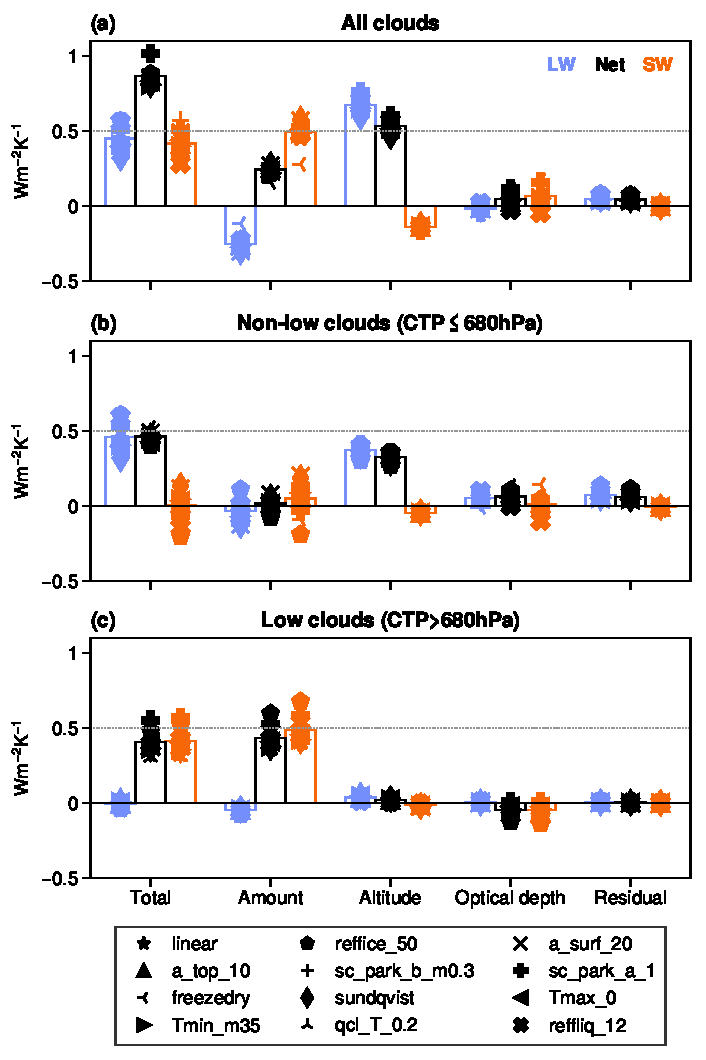
\includegraphics[width=0.6\linewidth]{{figs/change_of_CRE/global_mean_cld_fbk_decomp_scatter}.pdf}
    \caption{Global mean (orange) shortwave (SW), (blue) longwave (LW), and (black) net cloud feedbacks decomposed into amount, altitude, optical depth, and residual components for (a) all clouds, (b) non-low clouds (cloud top pressure, CTP$\le$680 hPa ), and (c) low clouds (CTP > 680hPa). The mean feedbacks of perturbed parameter ensemble are shown as empty bars.}
    \label{fig:global_mean_cld_fbk_scatter}
\end{figure}

The global mean longwave (light blue symbols), shortwave (oragne symbols), and net (black symbols) cloud feedbacks, and their non-low and low cloud components, are shown in \figref{fig:global_mean_cld_fbk_scatter}. For each cloud feedback, it is further broken down into amount, altitude and optical depth parts. As pointed by \cite{Zelinka2012computing2}, one can get total cloud feedback by summing its longwave and shortwave counterparts, which, however, does not hold for the feedback components. For example, you could not get the total cloud amount feedback by adding the low and non-low cloud amount feedbacks directly.

% Describe the global mean cloud feedback results of PPE
In all the runs of Isca PPE, the net non-low cloud altitude and net low cloud amount feedbacks are robustly positive (\figsref{fig:global_mean_cld_fbk_scatter}b and \ref{fig:global_mean_cld_fbk_scatter}c, black symbols), and the contributions are almost from one band (longwave or shortwave). Specifically, the positive low cloud amount feedback is due to its shortwave component, while the positive longwave part contributes most to the net non-low cloud altitude feedback. The former can be explained by the fact that the temperature difference between the cloud top of low clouds and surface is small, so the longwave effect of low clouds is insignificant compared to its shortwave counterpart. In contrast, for the non-low cloud altitude feedback, if the cloud amount and optical depth are fixed, the change of the altitude mainly effects the cloud top temperature, indicating that longwave effect plays an important role, which explains why the longwave component dominates the net non-low cloud feedback. Except these two components, the ensemble mean of other net cloud feedback components are close to zeros in the Isca PPE simulations (\figref{fig:global_mean_cld_fbk_scatter}), including the low cloud optical depth, a robust non-zero negative component in CMIP models \citep[e.g.,][]{Zelinka2016insights,Ceppi2017,Zelinka2020causes}. The reason for this missing feature is discussed in \secref{sec:spatial_pattern_cld_fbk}.

% On the contrary, the longwave component usually plays a more important role than the shortwave component for high clouds, 

The spread of net cloud feedback in Isca PPE is about 0.076 Wm$^{-2}$K$^{-1}$ (1$\sigma$), which is about 1/3 of the inter-model spread of CFMIP models \citep{Zelinka2016insights}. There are two possible reasons to explain why the spread in Isca PPE is lesser than the CFMIP intermodel uncertainty: First, the perturbation is limited to one parameter each time, and the parameter is limited within the simple cloud scheme itself. The range of the parameter space is rather narrow in current PPE of Isca. Second, only one model, Isca, is employed for the PPE, which is different from the CFMIP where models from multiple institutions are involved. In this case, the cloud schemes and other parameterization schemes may also contribute to the potential spread of cloud feedbacks. As previous study has pointed out that the responses in cloud fields under global warming are different for models with different cloud scheme \citep[e.g.,][]{Qu2014}, and replacing the cloud scheme in GCMs can reduce the inter-model spread of cloud feedback for CMIP5 models \citep{Geoffroy2017}. The net low cloud amount feedback exhibits greater uncertainty than the net cloud feedback, and the standard deviation is 0.077 Wm$^{-2}$K$^{-1}$. Although the non-low cloud altitude feedback is robust non-zero, its spread is relative small (standard deviation is 0.018 Wm$^{-2}$K$^{-1}$). In addition, the spread in non-low cloud amount feedback is about 0.041 Wm$^{-2}$K$^{-1}$, in spite of its ensemble mean is quite close to zero due to the cancellation between shortwave and longwave components (\figref{fig:global_mean_cld_fbk_scatter}b). In the next, we will evaluate their contributions quantitatively.

% Quantify the uncertainty of the spread of cloud feedbacks among the PPE
\begin{figure}[ht]
    \centering
    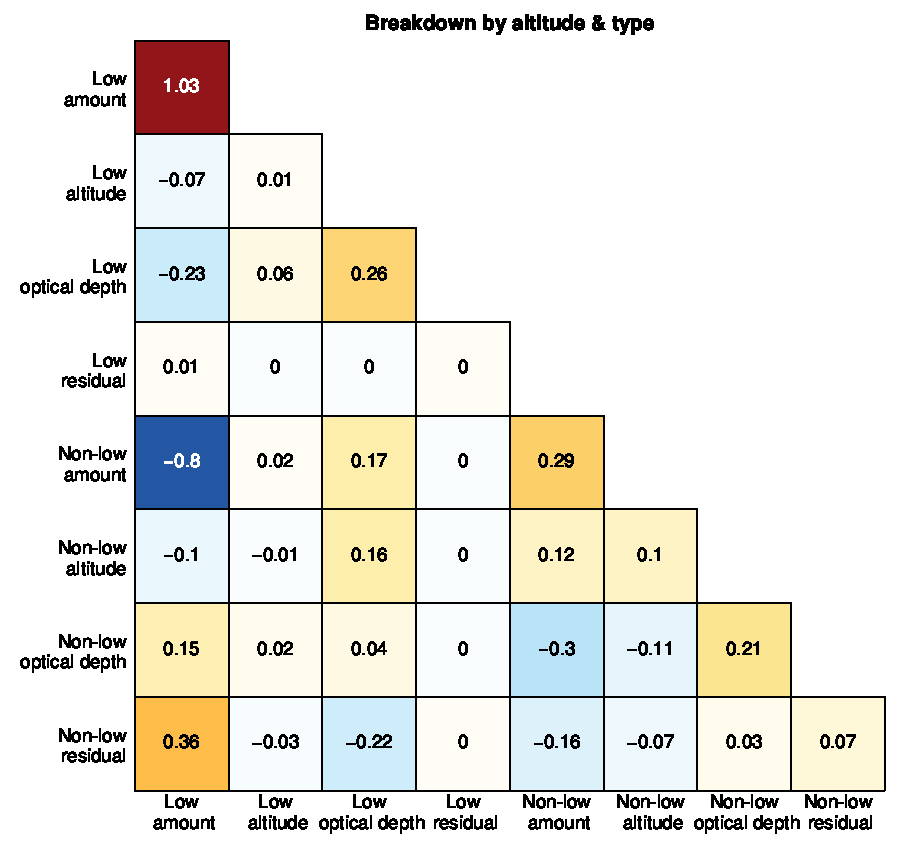
\includegraphics[width=0.9\linewidth]{{figs/change_of_CRE/covariance_contribution_breakdown_with_err}.pdf}
    \caption{The fractional contributions to the Isca perturbed physical ensemble variance in net cloud feedback are broken down to different altitudes and types, including low/non-low cloud amount, altitude, optical depth feedbacks and residuals.}
    \label{fig:variance_contribution_to_cld_fbks}
\end{figure}

Following \cite{Caldwell2016quantifying} and \cite{Zelinka2016insights}, the contribution of cloud types to the spread of net cloud cloud feedback is quantified as follows:

\begin{equation}
    \begin{aligned}
    \operatorname{var}\left(\sum_{i=1}^{N} X_{i}\right) &=\sum_{i=1}^{N} \sum_{j=1}^{N} \operatorname{cov}\left(X_{i}, X_{j}\right) \\
    &=\sum_{i=1}^{N} \operatorname{var}\left(X_{i}\right)+2 \sum_{j=1}^{N} \sum_{k=j+1}^{N} \operatorname{cov}\left(X_{i}, X_{j}\right),
    \end{aligned}
    \label{eq:cld_fbk_variance}
\end{equation}
where $X_i$ are low/non-low cloud amount, altitude, optical depth feedbacks and residuals in the decomposition. Then the ratios of these components to total variance are obtained and plotted in \figref{fig:variance_contribution_to_cld_fbks}. The the variance terms of each component are on the main diagonal, while the values below the diagonal are for the covariances terms. Here the covariance terms are multiplied by 2, so the section above diagonal in \figref{fig:variance_contribution_to_cld_fbks} is omitted. This is reasonable as the covariance matrix is symmetric and each covariance should be included twice, as indicated by \eqref{eq:cld_fbk_variance}. Covariance terms can be positive or negative while variances are always non-negative. 

The low cloud amount feedback is by far the largest single contributor to the spread of net cloud feedback in the Isca PPE, as indicated by the greatest variance ratio in \figref{fig:variance_contribution_to_cld_fbks}. It seems that the variance of low cloud amount feedback is even larger than that of total net cloud feedback in Isca PPE. This conclusion is qualitatively consistent with the results from CFMIP models that low cloud amount feedback contributes most to the net cloud feedback \citep[][]{Zelinka2016insights}. The second largest contributor is the non-low cloud amount feedback, which accounts for 29\% of the total variance of the net cloud feedback. But it also appears that there is a strong anticorrelation between the low cloud amount and non-low cloud amount feedbacks ($r=-0.73$), which reduces the spread of net cloud feedbacks, but the physical mechanism still needs further investigation. This anti-correlation is also found in CFMIP models, but \cite{Zelinka2016insights} thought it might be ``entirely fortuitous" as it is uncorrelated with non-low cloud fraction changes and there is no strong correlation between low and non-low cloud amount changes in the CFMIP models. The contribution from low-cloud optical depth feedback is also a relative important contributor to the spread of net cloud feedbacks, despite its ensemble mean is close to zero in Isca simulations.

% Todo: check the correlation between non-low cloud amount feedback with non-low cloud fraction changes in Isca
% In Isca simulations, we do find a strong anti-correlation between low cloud amount and high cloud amount changes in ISCCP diagnostics ($r=-$), but this does not exist in the native model outputs, indicating that the diagnostics may have some biases...

\subsection{Comparison with WCRP assessment}
\label{sec:cmp_with_Sherwood_assessment}

\begin{figure}[ht]
    \centering
    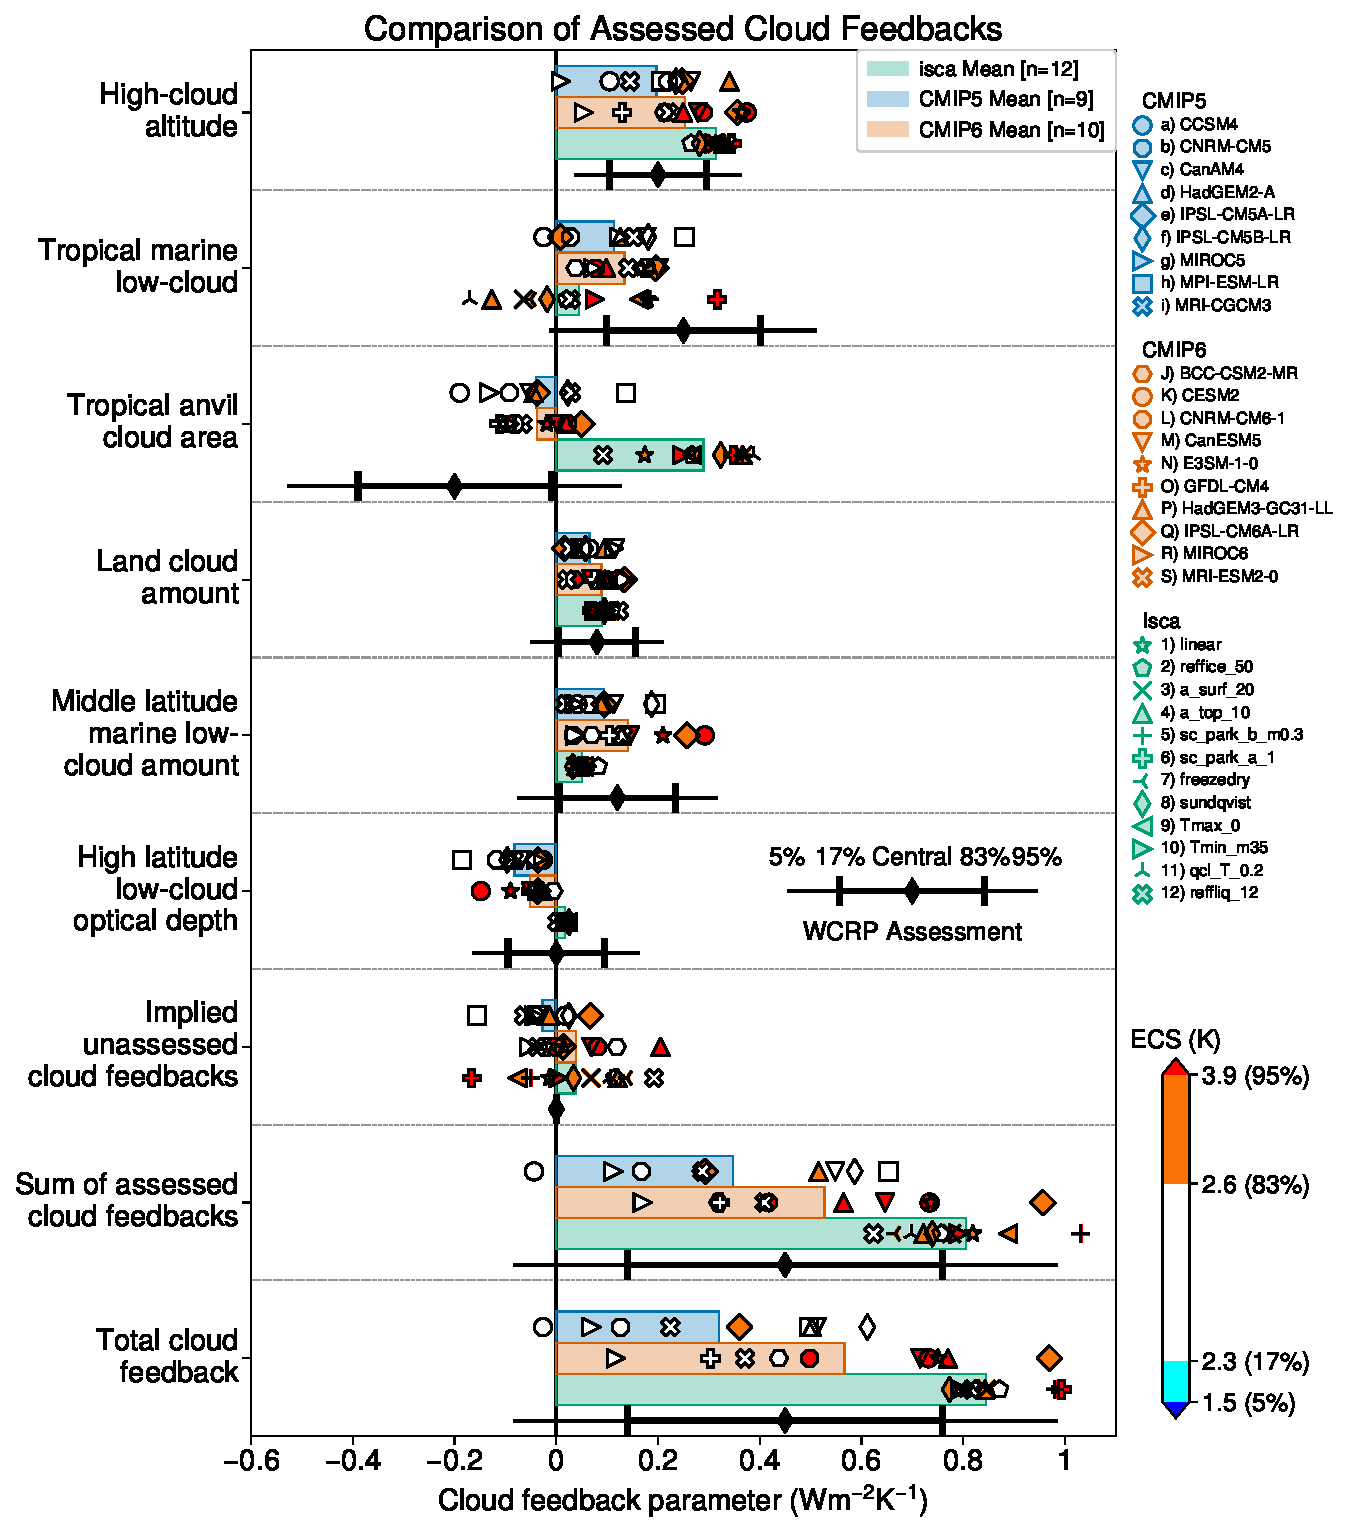
\includegraphics[width=0.81\linewidth]{{figs/change_of_CRE/WCRP_assessed_cld_fbks_amip-p4K}.pdf}
    \caption{Cloud feedback components estimated from climate model simulations and as assessed in \cite{Sherwood2020}. For each component, the individual model values are indicated with symbols, the multi-model means are indicated with blue (CMIP5), orange (CMIP6) and green (Isca) bars, and the expert assessed \textit{likely} (66\%, or 17\%--83\%) and \textit{very likely} (90\%, or 5\%--95\%) confidence intervals are indicated with thick and thin black errorbars, respectively. Model symbols (only for CMIP5/6) are color-coded by equilibrium climate sensivity (ECS) with color boundaries corresponding to the edges of the \textit{likely} (17\%--83\%) and \textit{very likely} (5\%--95\%) ranges of the Baseline posterior probability density function (PDF) of  ECS from \cite{Sherwood2020}. The results from Isca simulation are added to original Fig. 1 of \cite{Zelinka2021evaluating}.}
    \label{fig:WCRP_assessment}
\end{figure}

\cite{Zelinka2021evaluating} evaluated the cloud feedbacks from CMIP5 and CMIP6 models and compared them to the latest World Climate Research Programme (WCRP) assessment of cloud feedbacks reported in \cite{Sherwood2020}. Note that only 9 CMIP5 and 10 CMIP6 models are used, as only those that have successfully implemented the COSP \citep{BodasSalcedo2011} are adopted. Based on the analysis from \cite{Zelinka2021evaluating}, here the perturbed parameter ensemble simulations from Isca simulations are also added to this comparison, as shown in \figref{fig:WCRP_assessment}. In this figure, the feedback values from each category are weighted averaged according to their area fractions, so that the values shown in the last row of the figure are the direct sum of these categories. 

All the simulated cloud feedbacks from Isca are with the \textit{very likely} (90\%, or 5\%--95\%; thin black line of WCRP assessment) confidence intervals of expert assessment, except the ones related to tropical anvil cloud area and tropical marine low cloud. In Isca simulations, the tropical anvil cloud area feedback (third row) is computed as the sum of non-altitude related feedbacks from both low and high clouds in tropical deep convection region. Specifically, the sum includes low and high cloud mount and optical depth feedbacks. This feedback is strongly positive with the mean value larger than 0.3 Wm$^{-2}$K$^{-1}$, while the mean value of expert assessment is -0.2 Wm$^{-2}$K$^{-1}$ (1-$\sigma$ uncertainty is 0.2 Wm$^{-2}$K$^{-1}$). This feature makes the total cloud feedback from Isca simulations much positive, and are located at the right end of expert assessment (last row). Note that the CMIP5 and CMIP6 models also underestimate the magnitude of tropical anvil cloud area feedback, and some also produce the positive feedback parameters for this category. Nevertheless, their ensemble mean has the same negative sign as the expert assessment, although we notice it is very weak and close to zero. 

Regarding to the tropical marine low cloud feedback, the ensemble mean feedback from Isca simulation is much weaker than the expert assessed, and also weaker than the ensemble mean of CMIP5/6 models. Another feature of Isca simulation for this category is that the spread is quite large, and some member even produce the negative marine low cloud feedback. This is possibly due to...

%In addition, the \textit{likely} (66\%, or 17\%--83\%) and \textit{very likely} (90\%, or 5\%--95\%) confidence intervals from expert assessments of cloud feedbacks \citep[see Table 1 of][]{Sherwood2020} are indicated by the 

\figref{fig:WCRP_assessment} is produced using the software package developed by \cite{Zelinka2021evaluating}, available at \url{https://github.com/mzelinka/assessed-cloud-fbks}.

\subsection{Regional contributions}
\label{sec:reg_contri_to_spread_of_cldfbk}

\begin{figure}[ht]
    \centering
    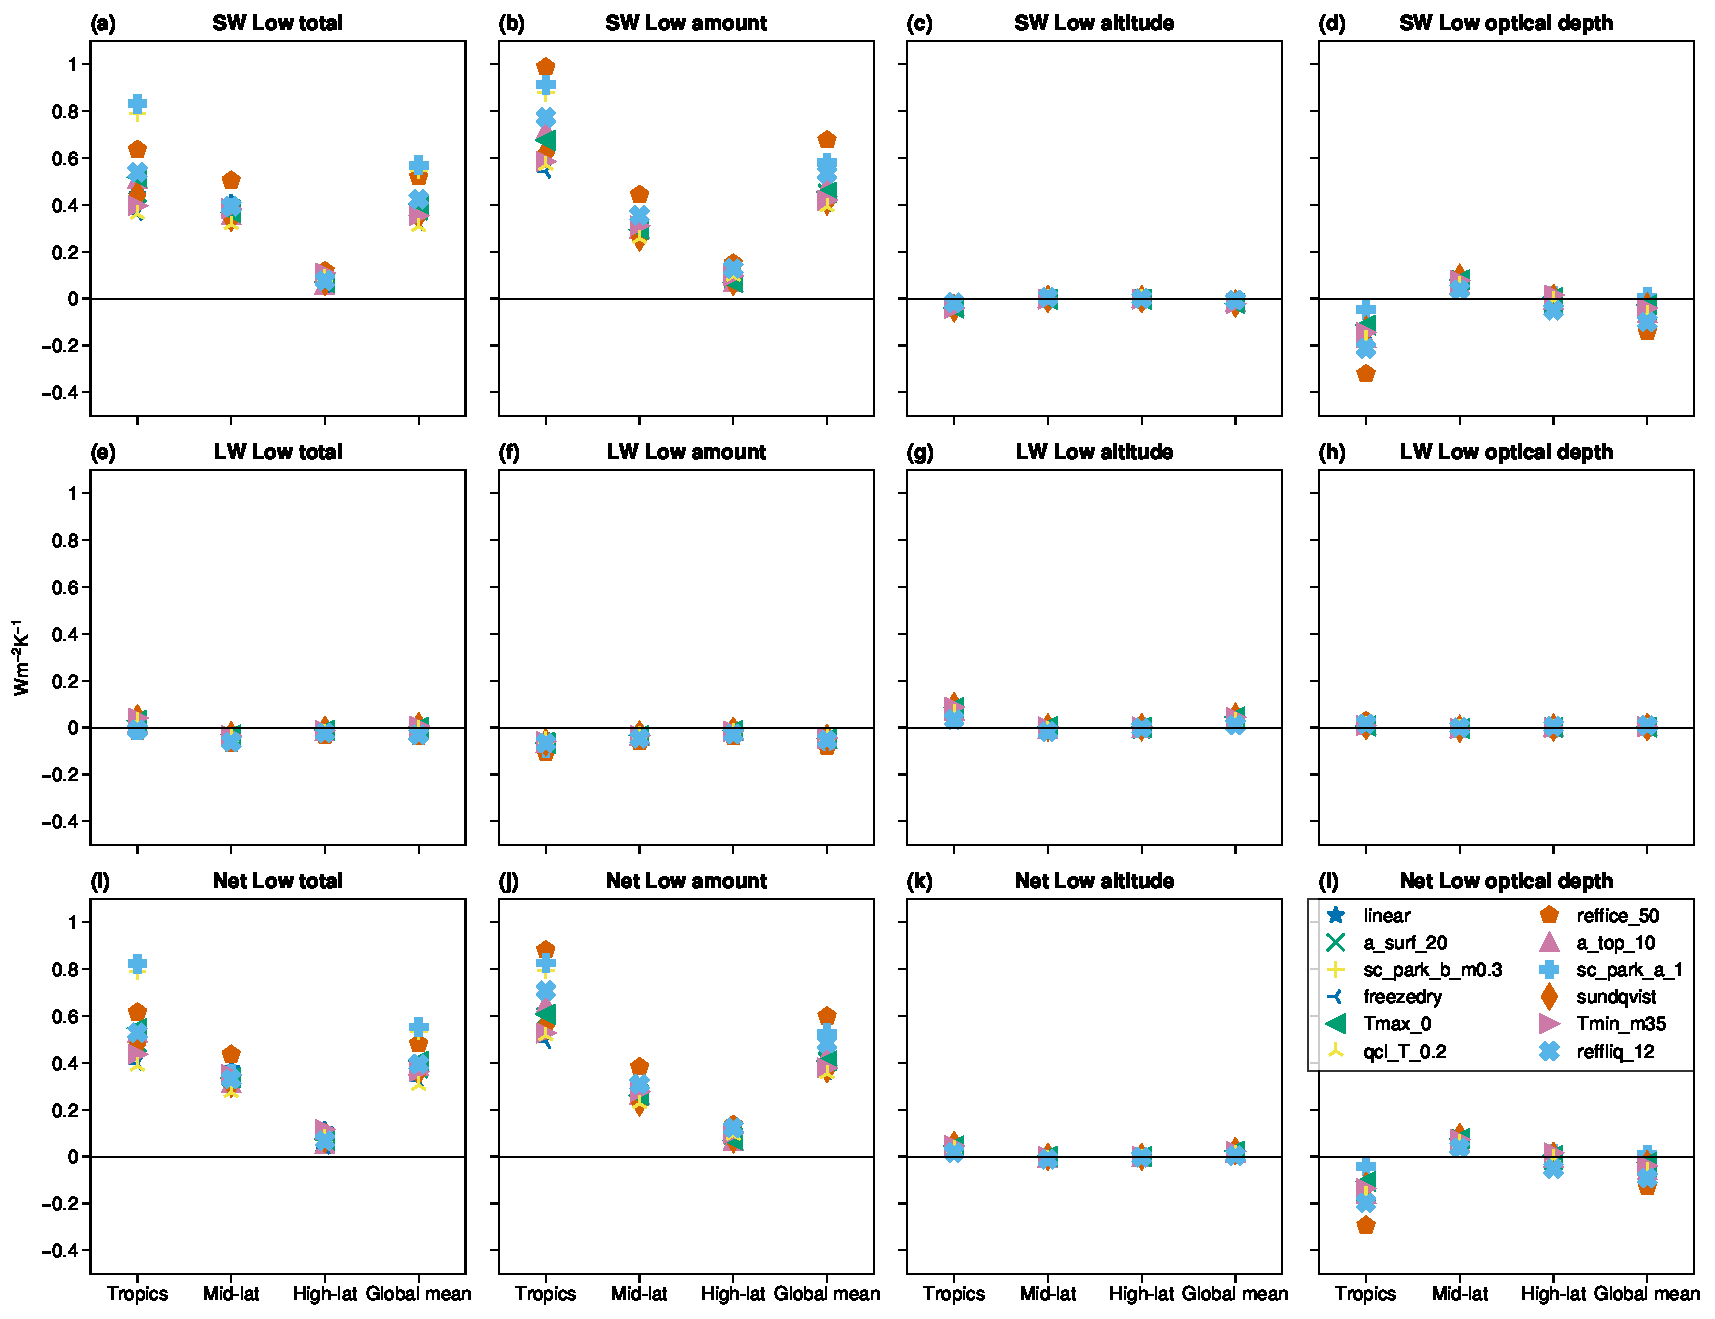
\includegraphics[width=1\linewidth]{{figs/change_of_CRE/region_mean_cld_fbk_decomp_scatter_LO680}.pdf}
    \caption{The scatter plot of total low cloud feedback (first column) and its amount (second column), altitude (third column) and optical depth (fourth column) components for different regions from Isca PPE. The top, middle and bottom rows are for the shortwave, longwave and net cloud feedbacks, respectively. }
    \label{fig:regional_low_cld_fbk_components}
\end{figure}

\secref{sec:spread_of_gm_cld_fbks_PPE} has found that the low cloud amount feedback is the largest single contributor to the spread of Isca PPE, but the analyses are based on the global mean values. This section extends the analysis to regional scales, and intends to identify which region has the largest uncertainty for low cloud feedback. \figref{fig:regional_low_cld_fbk_components} show the low cloud feedbacks and their various components in different regions, including tropics (30$^\circ$S--30$^\circ$N), midlatitudes (30$^\circ$--60$^\circ$S/N) and high latitudes (60$^\circ$--90$^\circ$S/N). Basically no matter in which regions, the longwave cloud feedback components (\figsref{fig:regional_low_cld_fbk_components}e--h) and the shortwave altitude feedback component (\figref{fig:regional_low_cld_fbk_components}c) are nearly zeros and contribute little to the spread of low cloud feedbacks in Isca PPE. In contrast, the shortwave cloud amount (\figref{fig:regional_low_cld_fbk_components}b) and optical depth (\figref{fig:regional_low_cld_fbk_components}c) feedbacks, especially the former, are the major sources of spread in low cloud feedbacks (see \figsref{fig:regional_low_cld_fbk_components}a and i). Focusing on the spread in different regions, we find the tropical region in fact plays the greatest part in determining the spread for global mean values of cloud feedbacks, both for cloud amount and optical depth components. As the spread in cloud amount feedback is larger that in optical depth, we can conclude that the tropical low cloud amount feedback (shortwave part) is the biggest contributor to the uncertainty of cloud feedback in Isca PPE, which is consistent with previous studies \citep[e.g.,][]{Bony2006}. 

\begin{figure}[ht]
    \centering
    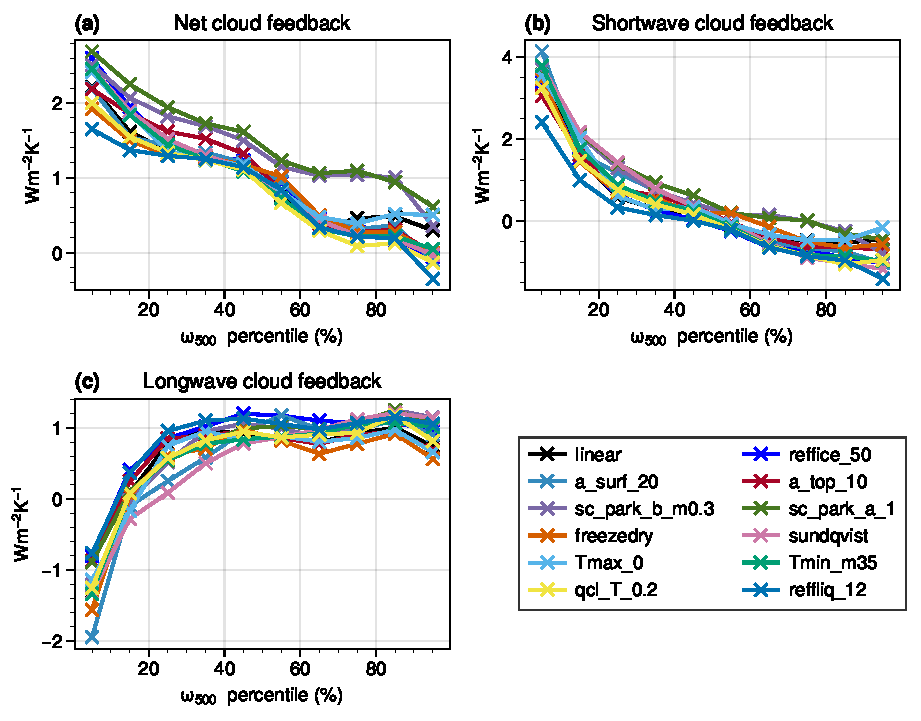
\includegraphics[width=0.8\linewidth]{{figs/change_of_CRE/cld_fbk_composited_by_omega500_percentile}.pdf}
    \caption{Composites of (a) net, (b) shortwave and (c) longwave cloud feedbacks over low-latitude oceans (30$^\circ$S--30$^\circ$N) in the Isca perturbed parameter ensemble, sorted by percentiles of the vertical velocity at 500 hPa ($\omega_{500}$). }
    \label{fig:cld_fbk_composite_w500_percentile}
\end{figure}

\begin{figure}[ht]
    \centering
    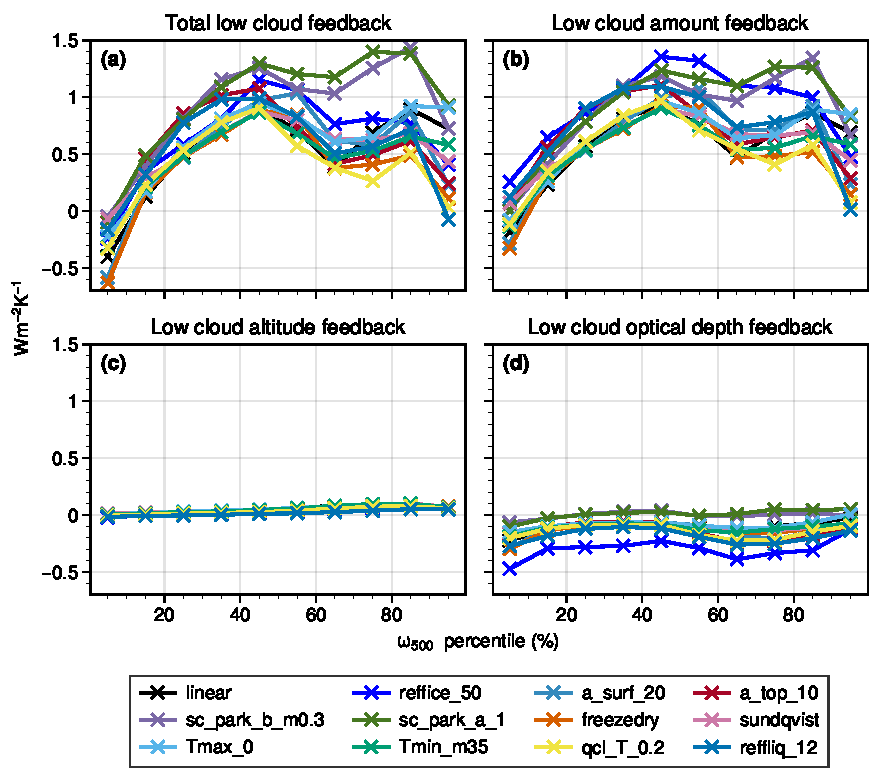
\includegraphics[width=0.8\linewidth]{{figs/change_of_CRE/low_cld_fbk_composited_by_omega500_percentile}.pdf}
    \caption{Similar to \figref{fig:cld_fbk_composite_w500_percentile}, but the composites for (a) the total low cloud feedback and its (b) amount, (c) altitude and (d) optical depth components.}
    \label{fig:low_cld_fbk_composite_w500_percentile}
\end{figure}

A further step from the above analysis is to divide the tropical region into different dynamical regimes. For example, \cite{Bony2004} has propose a method to decompose the tropical ocean region into ascending and subsidence regimes with the vertical velocity at 500 hPa ($\omega_{500}$), as these two regimes have distinctive dynamical and thermodynamical properties for clouds formation. This comosite analysis has been used in \chapref{ch:simple_cld_scheme} to evaluate the simulated longwave cloud radiative effect from simple cloud scheme in tropical regions. Here we apply this composite analysis again to assess the simulated cloud feedback in tropical regions, and seek to find which dynamical regime has the largest uncertainty in cloud feedbacks.

\figref{fig:cld_fbk_composite_w500_percentile} shows composites of cloud feedback over the low-latitude (30$^\circ$S--30$^\circ$N) oceans in the Isca PPE simulations, sorted by the percentiles of vertical velocity at 500 hPa ($\omega_{500}$). Note that the percentile rather than actual $\omega_{500}$ is used for analysis. Larger percentiles represent the subsidence regimes over tropical and subtropical regions, while lower percentiles represent the deep convection areas. The spread of net cloud feedback is large in large percentile regimes (\figref{fig:cld_fbk_composite_w500_percentile}a), which is from the shortwave component (\figref{fig:cld_fbk_composite_w500_percentile}b; Note the scales of y-axis are different in \figref{fig:cld_fbk_composite_w500_percentile}). As previous studies such as \cite{Bony2005} has found that the marine boundary layer clouds are at the heart of tropical cloud feedback uncertainties in climate models, we further carry out the composite analysis for low cloud feedback in tropical ocean regions (\figref{fig:low_cld_fbk_composite_w500_percentile}). It is noteworthy that the low cloud amount feedback shows the largest difference  over subsidence regions (percentiles greater than 50\%) among the Isca PPE (\figref{fig:low_cld_fbk_composite_w500_percentile}b), while the uncertainty in low cloud altitude and optical depth feedbacks are relatively low (\figsref{fig:low_cld_fbk_composite_w500_percentile}c and d). This finding confirms the results from \figref{fig:regional_low_cld_fbk_components} that tropical low cloud amount feedback is one of the largest source of uncertainty in net cloud feedback, and also identifies that the subsidence regime in fact plays a major role for low cloud feedback uncertainty, consistent with the findings from \cite{Bony2005}.

\subsection{Cloud controlling factor analysis}
\label{sec:cld_control_factor}

Why does the low cloud amount feedback have the largest uncertainty over the subsidence regions in Isca PPE simulations? To answer this question, the cloud controlling factor analysis \citep[e.g.,][]{Qu2015positive,Myers2016,McCoy2017change,Klein2017low,Scott2020,Myers2021,Cesana2021,Ceppi2021observational} is employed in this section to analyze the sensitivity of low cloud amount to various large-scale meteorological conditions. 

\begin{figure}[ht]
    \centering
    \includegraphics[width=0.8\linewidth]{{figs/change_of_CRE/regime_and_profiles_EIS_4.0}.png}
    \caption{(a) The frequency of occurrence for (blue) trade-wind cumulus clouds and (red) stratocumulus clouds in low-latitude (35$^\circ$S--35$^\circ$N) ocean regions. Stippled regions indicate both types of cloud regimes can occur, but the color is chosen as the more frequent one. (b--e) The vertical profile changes in (b) relative humidity, (c) temperature, (d) cloud fraction and (e) cloud water content in trade-wind cumulus cloud regions under global warming in Isca perturbed parameter ensemble simulations. (f--i) As in (b--e), but for stratocumulus regions.}
    \label{fig:trade_wind_Cu_and_Sc_region_partition_and_change_of_profs}
\end{figure}

In the tropical and subtropical regions, climate regimes usually contain different cloud types. To this end, it is better to partition the whole region into different cloud regimes. In fact, several metrics have been proposed to partition the cloud regimes. For example, \cite{Medeiros2011} combined the vertical velocity at 500/700 hPa ($\omega_{500}$ or $\omega_{700}$) and lower tropospheric stability (LTS) to partition the trade-wind cumulus clouds (Cu) and stratocumulus (Sc) over topical oceans. Recently, the metric such as estimate inversion strength (EIS) is also adopted for same purpose in latest studies \citep{Scott2020,Myers2021,Cesana2021}. In a similar manner as \cite{Scott2020}, the criterion to partition the low cloud regimes over tropical oceans are as follows: the regimes are trade-wind cumulus clouds if $\omega_{700}>15$ hPa and EIS $<4$ K, and the regimes are stratocumulus clouds if $\omega_{700}>15$ hPa and EIS $\geq 4$ K. The first criteria ($\omega_{700}$) is to make sure the clouds are in the subsidence regime and the second one (EIS) is to distinguish different low cloud types. An example of this partition is shown in \figref{fig:trade_wind_Cu_and_Sc_region_partition_and_change_of_profs}a, in which the blue denotes the frequency of occurrence of trade-wind cumulus clouds, while the red represents the frequency of occurrence of stratocumulus clouds. Stippled regions indicate both types of cloud regimes can occur, but the color is chosen as the more frequent one. As we have discussed in \chapref{ch:simple_cld_scheme}, the statocumulus clouds are abundant in subtropical oceans off the west coast of continents (\figref{fig:trade_wind_Cu_and_Sc_region_partition_and_change_of_profs}a). 

Under global warming, the changes of lower tropospheric cloud fraction profiles over trade-wind cumulus and stratocumulus cloud regimes in low-latitude oceans are different in Isca PPE control and 4$\times$CO$_2$ simulations (\figsref{fig:trade_wind_Cu_and_Sc_region_partition_and_change_of_profs}d and \ref{fig:trade_wind_Cu_and_Sc_region_partition_and_change_of_profs}h). The cloud fractions in lower troposphere show clear reduction in trade-wind cumulus cloud region (\figref{fig:trade_wind_Cu_and_Sc_region_partition_and_change_of_profs}d), which is consistent with the decrease in relative humidity at the same locations (\figref{fig:trade_wind_Cu_and_Sc_region_partition_and_change_of_profs}b). In contrast, the cloud fractions over stratocumulus cloud regime increase in lower troposphere (\figref{fig:trade_wind_Cu_and_Sc_region_partition_and_change_of_profs}h), in despite of the reduction in relative humidity (\figref{fig:trade_wind_Cu_and_Sc_region_partition_and_change_of_profs}f). The inconsistency in stratocumulus cloud regime is due to the fact that the marine low clouds, particularly the stratocumulus clouds, are not directly diagnosed from relative humidity, but also from the inversion strength related variable. As introduced in \secref{sec:marine_low_cld_scheme}, the maximum of the two diagnoses is regarded as the cloud fraction over stratocumulus cloud region. Therefore, the increase of cloud fraction over stratocumulus regime may reflect the strengthened inversion strength there \citep[e.g.,][]{Webb2013origins,Webb2018interactions}.

% EIS changes
\begin{figure}[ht]
    \centering
    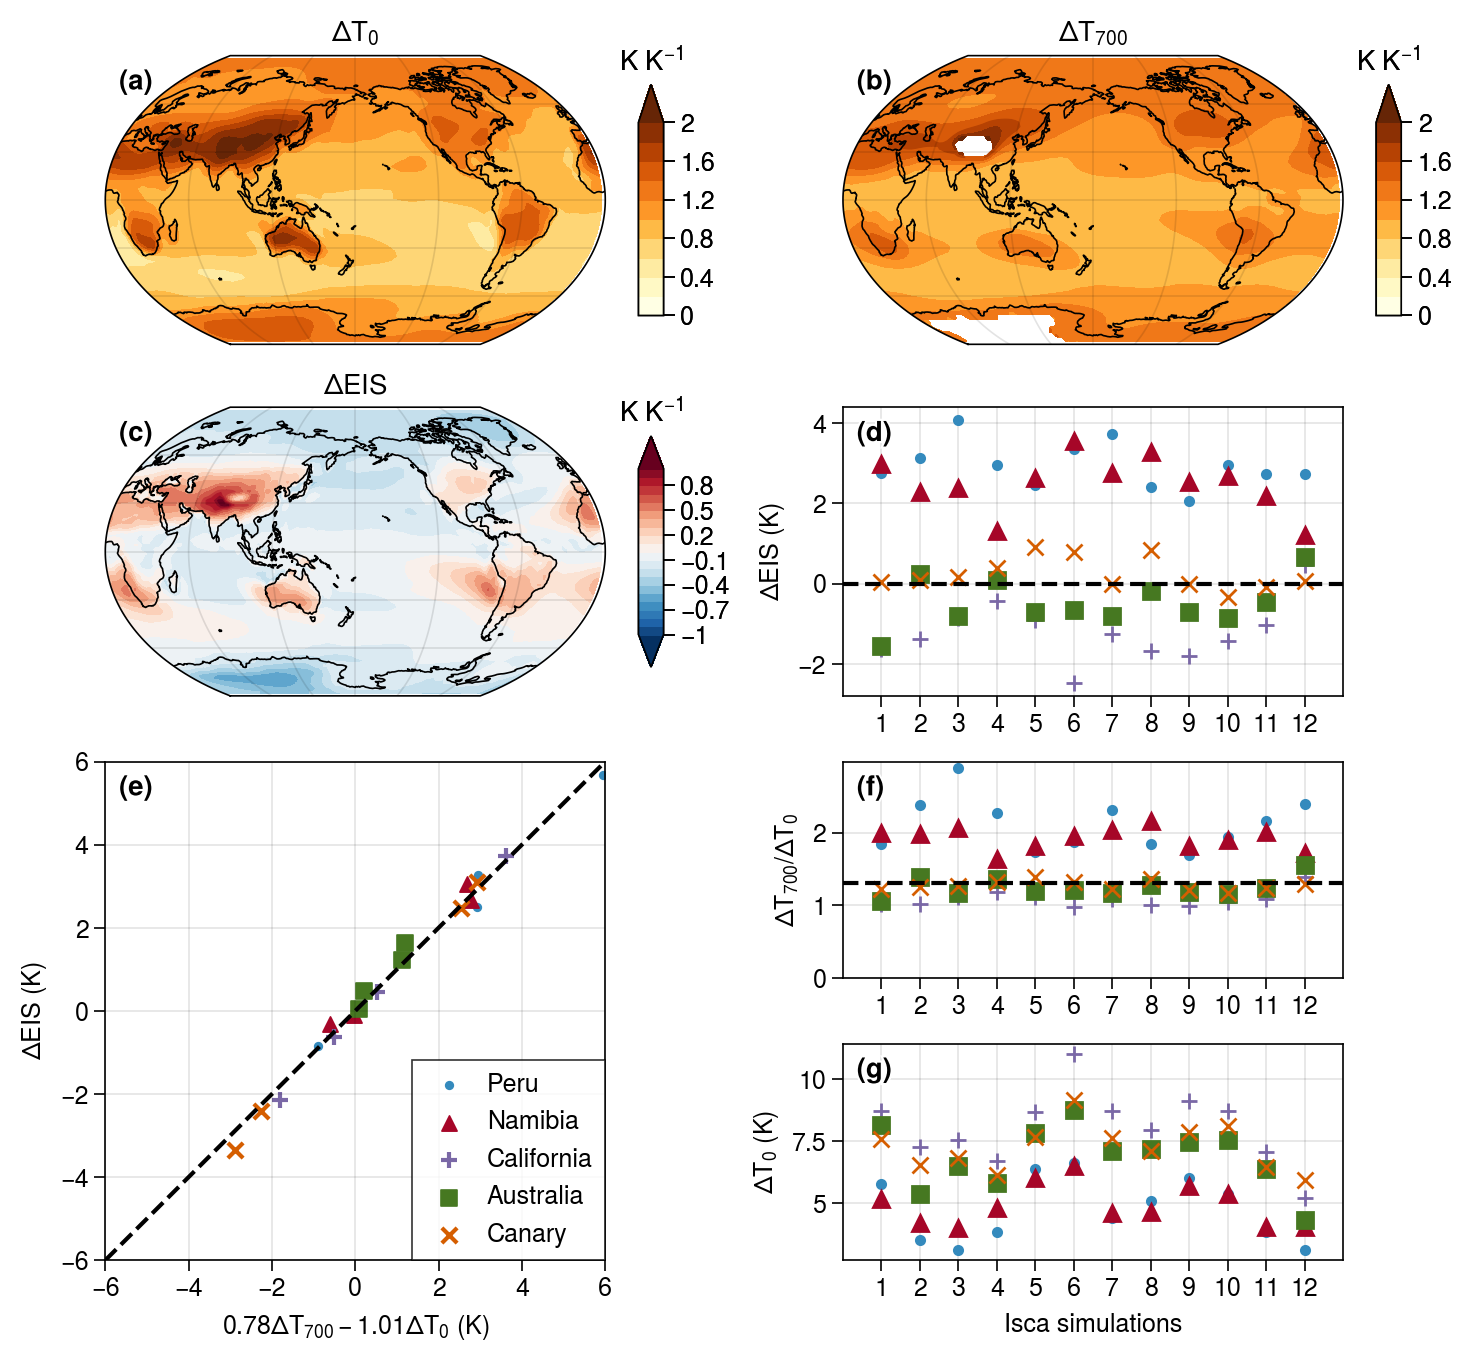
\includegraphics[width=0.85\linewidth]{{figs/change_of_CRE/EIS_change_pattern_and_estimation}.png}
    \caption{The annual and ensemble mean changes in (a) surface air temperature ($T_{0}$), (b) temperature at 700 hPa ($T_{700}$) and (c) estimate inversion strength (EIS) in Isca perturbed parameter ensemble (PPE) simulations, and these changes are normalized by the global mean surface air temperature. (e) The seasonal mean changes in EIS are estimated by the changes in surface temperature and temperature at 700 hPa for five marine low cloud regions in Isca simulation. The annual and regional mean EIS changes, the ratio between changes in $T_{700}$ and $T_0$, and surface temperature changes for each member of Isca PPE are shown in (d), (f) and (g), respectively. The ranges of the five locations are the same as those used in \figref{fig:fit_low_cld_proxy}. }
    \label{fig:EIS_changes_in_Isca_PPE}
\end{figure}

To check the changes of EIS under global warming, the ensemble mean spatial patterns of changes in surface temperature, temperature at free troposphere, and EIS in Isca PPE simulations are shown in \figsref{fig:EIS_changes_in_Isca_PPE}a, b and c, respectively, and these changes are normalized by the gloabl mean surface air temperature changes. Focusing on the stratocumulus regimes over the subtropical eastern Pacific region, we can find the surface warming (\figref{fig:EIS_changes_in_Isca_PPE}a) is relative lower than the warming at 700 hPa (\figref{fig:EIS_changes_in_Isca_PPE}b), and this perhaps could explain the increase of EIS there (\figref{fig:EIS_changes_in_Isca_PPE}c). The reason is that the change of EIS can be approximately explained by the changes of surface temperature ($\Delta T_0$) and temperature at 700 hPa ($\Delta T_{700}$), as pointed by \cite{Qu2014} (see the analytical expression for EIS change in their Appendix 2). Basically, following the mosit adiabatic assumption and with some simplifications, the change of EIS can be written as:
\begin{equation}
    \Delta\text{EIS} =\alpha \Delta T_{700} - \beta \Delta T_0,
    \label{eq:eis_change_T0_T700}
\end{equation}
where the linear coefficients $\alpha$ and $\beta$ are positive values and can be derived theoretically or obtained by regressing the model data. In this case, EIS increases if the ratio between the warming at 700 hPa and surface ($\Delta T_{700}/\Delta T_0$) is larger than certain threshold (i.e., $\beta/\alpha$). In other words, $\Delta$EIS $\geq 0$ if $\Delta T_{700}/\Delta T_0\geq \beta/\alpha$. To verify this relationship, the seasonal changes of EIS, $T_{700}$ and $T_{0}$ from five marine low cloud regions \citep{Klein1993,Qu2014} in a pair of control and 4$\times$CO$_2$ Isca simulations are selected to derive their relationship and linear coefficients in \Eqref{eq:eis_change_T0_T700}, with the result displayed in \figref{fig:EIS_changes_in_Isca_PPE}e (Note that the constant, or the y-axis intercept, in the relationship is neglected in plotting). Thus, the change of EIS in Isca simulations can be estimated by $\Delta$EIS $\approx 0.78\Delta T_{700} - 1.01\Delta T_0$, and $\Delta$EIS $>0$ if it is greater than $1.01/.78\approx1.29$, close to the theoretical ratio (1.18) in \cite{Qu2014}. This conclusion holds if the derived relationship is applied to all the Isca PPE simulations (\figsref{fig:EIS_changes_in_Isca_PPE}d, f and g). It is clear that the annual mean changes of EIS are positive (\figref{fig:EIS_changes_in_Isca_PPE}d) if the temperature warming ratio between 700 hPa and surface is larger than 1.29, as denoted by the horizontal dashed line in \figref{fig:EIS_changes_in_Isca_PPE}f. 

According to \cite{Wood2006}, $\Delta$EIS is close to zero if the vertical profile of tropospheric warming follows a moist adiabat from the subtropical surface ($\Delta T_{700}/\Delta T_0\approx 1.2$). Therefore, it is the greater-than-adiabatic warming in subtropical free troposphere that leads to the more stable environment \citep{Qu2014}. There are two possible reason for this: The first is the uneven warming pattern in tropical and subtropical regions, as indicated by the surface temperature warming pattern in \figref{fig:EIS_changes_in_Isca_PPE}a, in which the warming in tropical west Pacific is enhanced than subtropical low cloud regions. Based on the weak-temperature gradient approximation \citep{Sobel2001weak}, the low-latitude free troposphere temperature is largely set by the warm pool region, so the enhanced warming in west Pacific could lead to the free tropospheric temperature warming in subtropical low cloud regions \citep[e.g.][]{Zhou2016,Zhou2017,Mauritsen2016clouds,McCoy2017change,Andrews2018,Dong2019attributing}. The second is probably due to the rapid warming over nearby land \citep{Qu2014,Qu2015strength}. As indicated in \figref{fig:EIS_changes_in_Isca_PPE}b, in the marine low cloud regions, the land temperature changes are larger than the nearby ocean region in free troposphere.

\begin{figure}[ht]
    \centering
    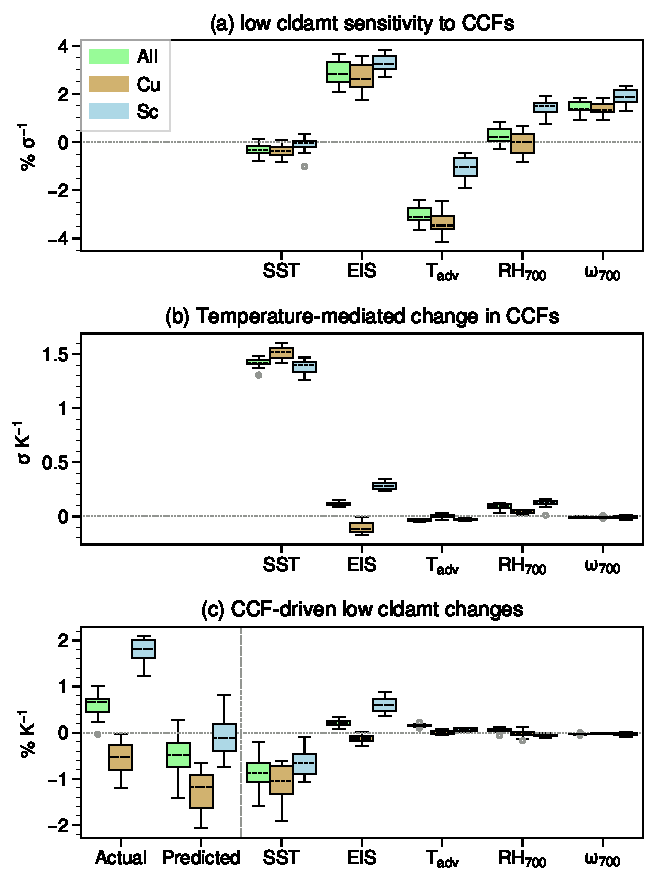
\includegraphics[width=0.6\linewidth]{{figs/change_of_CRE/CCF_analysis_for_diff_cld_types_low_cld_amt_EIS}.pdf}
    \caption{(a) Sensitivities of trade-wind cumulus (Cu; brown box), stratocumulus (Sc; blue box) and all low cloud amounts (green box) to cloud controlling factors (CCF), including sea surface temperature (SST), estimated inversion strength (EIS), surface temperature advection (T$_{adv}$), relative humidity at 700 hPa (RH$_{700}$), and vertical velocity at 700 hPa ($\omega_{700}$) estimated from climate variability over low-latitude oceans (35$^\circ$S--35$^\circ$N) the in the control simulations of Isca perturbed parameter ensemble. (b) The changes in these factors per unit global warming from the 4xCO2 simulations of Isca. (c) Predicted and actual changes in low cloud amount due to each cloud controlling factor. Boxes extend from the 25th to 75th percentiles of the model values, with a dashed line at the median value. Outliers are denoted by gray empty circles. Anomalies in cloud controlling factors are normalized by the standard deviation of their interannual variations in ERA5 data set and are therefore expressed in $\sigma$ units.} % , estimated as the product of the sensitivities shown in (a) with the responses of the quantities in (b)
    \label{fig:CCF_analysis_low_cld_amt}
\end{figure}

The above analyses put emphasis on EIS, which is one of the key meteorological factors that could help us understand the change of low cloud changes. As EIS increases, the strengthened inversion strength inhibits the mixing between moist boundary with the drying free troposphere, in favor of more low clouds \citep[e.g.,][]{Qu2014,Qu2015strength,Ceppi2017,Webb2018interactions,Scott2020}. Actually, the other cloud controlling factors such as sea surface temperature (SST) also contribute to the low cloud field changes, and may have opposite effects from EIS \citep[e.g.,][]{Bretherton2015,Myers2016,Scott2020,Myers2021,Cesana2021}. As summarized in \cite{Klein2017low}, many different predictor variables have been used in previous studies. In this section, following the analysis in \cite{Myers2016} and \cite{Zelinka2020causes}, we use the SST, EIS, temperature advection (T$_{adv}$), relative humidity in free troposphere at 700 hPa (RH$_{700}$) and vertical velocity at 700 hPa ($\omega_{700}$) to build the multiple linear regression model, with the results displayed in \figref{fig:CCF_analysis_low_cld_amt}. The analyses are performed over the trade-wind cumulus, stratocumulus and all low cloud regimes over tropical ocean regions (35$^\circ$S/N), respectively. The anomalies of the meteorological factors in Isca outputs are normalized by the standard deviation of climatology data set from ERA5 \citep{era5}, covering the period from 1979 to 2018. Moreover, we need to keep in mind that some of the meteorological factors might co-vary and not be independent with each other, such as SST and EIS \citep{McCoy2017change}, which might bring some problems in explaining the predicted results.



In Isca simulations, the dependence of low cloud amount on SST is negative (\figref{fig:CCF_analysis_low_cld_amt}a) for both trade-wind cumulus and stratocumulus cloud regimes, although the sensitivity of stratocumulus region is much weaker. This negative dependence is consistent with previous large-eddy simulation (LES) studies \citep[e.g.,][]{Bretherton2015}, observational studies \citep[e.g.,][]{Qu2015positive,Seethala2015,Scott2020,Myers2021} and GCM studies \citep[e.g.,][]{Myers2016}. The mechanism for this negative sensitivity is as follows: warmer SST increases the moisture in the boundary layer, which releases more latent heat flux and thus enhances the mixing with the free tropospheric dry air, thereby favoring less low clouds \citep{Qu2015positive,Scott2020}. As the SST increases under global warming for both two cloud regimes (SST column in \figref{fig:CCF_analysis_low_cld_amt}b), the final SST-driven low cloud amount changes are negative for all the cloud regimes (SST column in \figref{fig:CCF_analysis_low_cld_amt}c).

In contrast, the effect of EIS on low cloud amount is opposite to SST, as shown in the EIS column of \figref{fig:CCF_analysis_low_cld_amt}a. This is because stronger inversion strength of boundary layer inhibits the entrainment drying at the cloud top and thus favors the formation of low clouds \cite[e.g.,][]{Bretherton2015,Scott2020}. The positive dependence of low cloud amount on EIS in Isca simulation is also consistent with previous studies \citep{Qu2015positive,Myers2021,Cesana2021}, and this positive dependence holds for both trade-wind cumulus and stratocumulus regimes. However, we find the EIS changes in these two cloud regimes are different under global warming in Isca simulations. EIS increases in stratocumulus cloud regime while decreases in trade-wind cumulus cloud regime, which can be inferred from the EIS changes in \figref{fig:EIS_changes_in_Isca_PPE}c. Therefore, low cloud amount changes driven by EIS are opposite for these two regimes (see EIS column in \figref{fig:CCF_analysis_low_cld_amt}c). For all the low clouds, the EIS-driven amount changes are weakly positive.

In terms of the other factors such as T$_{adv}$, RH$_{700}$ and $\omega_{700}$, their changes under global warming in Isca simulations are small (the last three columns in \figref{fig:CCF_analysis_low_cld_amt}b), and thus the final contributions to low cloud amount change are neglected compared to the contributions from SST and EIS, as shown in \figref{fig:CCF_analysis_low_cld_amt}c. The negative sensitivity of low cloud amount to T$_{adv}$ is well simulated in Isca (third column in \figref{fig:CCF_analysis_low_cld_amt}a), as positive T$_{adv}$ brings relatively warm and moist air over cooler water, which stabilizes the boundary layer and cuts off clouds from the surface moisture supply \citep{Scott2020}. But we should note that Isca does not seem to be able to grasp the dependence of low cloud amount changes on $\omega_{700}$, showing positive dependence on it, while other studies show a negative dependence \citep[e.g.,][]{Scott2020,Zelinka2020causes}, as the LES simulation shows the thinning of low clouds under strong subsidence \citep{Bretherton2015}. However, we find this negative dependence of low cloud amount on $\omega_{700}$ can be simulated well for total cloud amount in Isca (not shown). It is possible that the simple diagnostic cloud scheme introduced in \chapref{ch:simple_cld_scheme} could not grasp the physical mechanisms found in LES. But as pointed by \cite{McCoy2017change}, this mechanism also seems to be regime and model dependent, and also given the contributions from $\omega_{700}$ to final low cloud amount change in Isca simulation are tiny, we do not need to worry too much about this problem in the simple cloud scheme of Isca.

For the sum of the low cloud amount changes under global warming in Isca simulations (first two columns of \figref{fig:CCF_analysis_low_cld_amt}c), we find the SST and EIS are the major contributors to the these changes, in agreement with previous studies \citep{Myers2015relationships,Myers2016,Qu2015positive,Seethala2015,Zhou2015,McCoy2016relationships}. For trade-wind cumulus cloud regime, the sum of CCF-driven cloud amount changes is negative, suggesting the reduction of cumulus clouds under global warming. Also, the predicted changes of cumulus clouds is close to the actual changes in Isca simulation (first column in \figref{fig:CCF_analysis_low_cld_amt}c), in agreement with the reduction of cloud fraction in lower troposphere shown in \figref{fig:EIS_changes_in_Isca_PPE}d. For the stratocumulus clouds, the mean value of sum of CCF-driven cloud amount changes is close to zero (second column in \figref{fig:CCF_analysis_low_cld_amt}c), while the actual changes in Isca simulations are much positive (first column in \figref{fig:CCF_analysis_low_cld_amt}c). This discrepancy is probably because the simple cloud scheme for stratocumulus regime is too strongly dependent on the inversion strength, while the multiple linear model overestimates its dependence on SST. We notice that such prediction among GCMs is also not so good, and thus some studies try to use observation to constrain the predictions \citep{Myers2016,Myers2021}. 

In fact, despite the prediction from the multiple linear regression model is not as good as expected, we still can get some useful ideas on the uncertainty of cloud feedback among Isca PPE simulations. It is noted that compared to the low cloud amount changes driven by EIS and other cloud controlling factors, the responses to SST show the largest spread,  (\figref{fig:CCF_analysis_low_cld_amt}c). This implies that the spread of low cloud amount changes are probably largely determined by SST-related changes, which is perhaps resulting from the radiative effect changes due to perturbed parameters in cloud scheme.

\section{Implications for equilibrium climate sensitivity}
\label{sec:implification_for_ECS}

% \begin{figure}[ht]
%     \centering
%     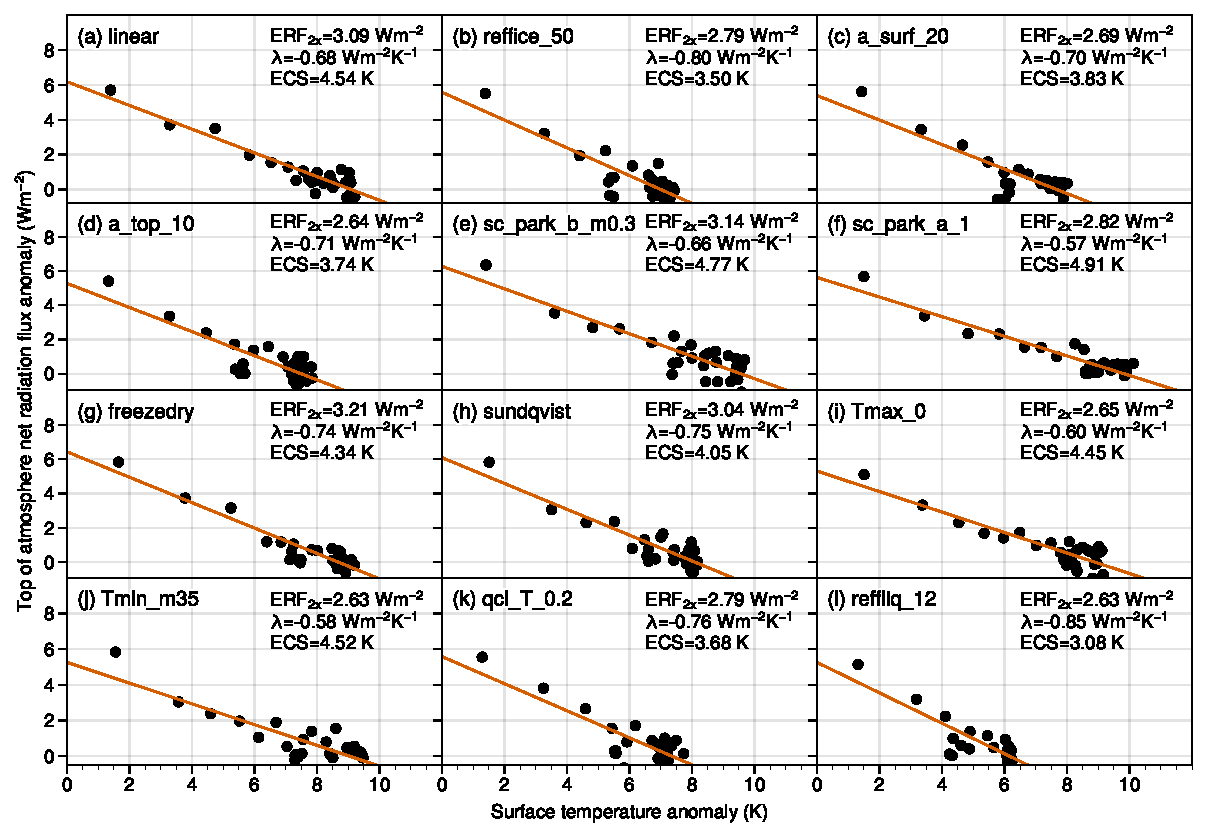
\includegraphics[width=0.9\linewidth]{{figs/change_of_CRE/forcing_slope_ECS_for_qflux_PPE_nyr_30_12}.pdf}
%     \caption{The effective radiative forcing, climate feedback and equilibrium climate sensitivity (ECS) in Isca perturbed parameter ensemble, estimated from the \cite{Gregory2004} method based on 30-year outputs.}
%     \label{fig:ECS_forcing_feedback_in_Isca_PPE}
% \end{figure}


 \begin{table}[ht]
    %\begin{sidewaystable}
	\caption{Effective radiative forcing (ERF$_{2x}$, Wm$^{-2}$), equilibrium climate sensitivity (ECS, K) and climate feedback parameters ($\lambda$, Wm$^{-2}$K$^{-1}$) for Isca perturbed parameter ensemble simulations.}
	\centering
	\renewcommand{\arraystretch}{1.2}

    \begin{tabular}{lrrrrrr}
    \toprule
    {PPE} &  ERF$_{2x}$ &  $\lambda$ &  $\lambda_{cld}$ &  $\lambda_{cld\_SW}$ &  $\lambda_{cld\_LW}$ &  ECS \\
    \midrule
    linear         &    3.09 &   -0.68 &        0.81 &           0.39 &           0.42 & 4.54 \\
    reffice\_50     &    2.79 &   -0.80 &        0.88 &           0.32 &           0.56 & 3.50 \\
    a\_surf\_20      &    2.69 &   -0.70 &        0.85 &           0.48 &           0.37 & 3.83 \\
    a\_top\_10       &    2.64 &   -0.71 &        0.85 &           0.41 &           0.44 & 3.74 \\
    sc\_park\_b\_m0.3 &    3.14 &   -0.66 &        0.98 &           0.54 &           0.45 & 4.77 \\
    sc\_park\_a\_1    &    2.82 &   -0.57 &        1.00 &           0.50 &           0.50 & 4.91 \\
    freezedry      &    3.21 &   -0.74 &        0.81 &           0.31 &           0.50 & 4.34 \\
    sundqvist      &    3.04 &   -0.75 &        0.78 &           0.46 &           0.32 & 4.05 \\
    Tmax\_0         &    2.65 &   -0.60 &        0.82 &           0.43 &           0.39 & 4.45 \\
    Tmin\_m35       &    2.63 &   -0.58 &        0.80 &           0.39 &           0.41 & 4.52 \\
    qcl\_T\_0.2      &    2.79 &   -0.76 &        0.81 &           0.42 &           0.39 & 3.68 \\
    reffliq\_12     &    2.63 &   -0.85 &        0.82 &           0.29 &           0.53 & 3.08 \\
    \bottomrule
    \label{tab:ECS_forcing_feedback}
    \end{tabular}
\end{table}

The Isca PPE simulations have produced a certain range in cloud feedbacks, as discussed in \secref{sec:spread_of_cld_fbk_in_PPE} and also in \tabref{tab:ECS_forcing_feedback}, so what are the implications for the ECS? To answer this question, we first evaluate the ECS from Isca simulations based on the method proposed by \cite{Gregory2004}. That is to say, the TOA radiation imbalances are plotted versus the surface air temperature anomalies between control and quadruple CO$_2$ simulations, in which the half of the x-axis intercept is the ECS, as the effective radiative forcing is defined in double CO$_2$ situation. The other derived parameters, climate feedback parameter ($\lambda$; slope) and effective radiative forcing (half of the y-axis intercept), are shown in \tabref{tab:ECS_forcing_feedback}. The Gregory type calculation is possible in current Q-flux setup as the SST can vary in response to the changes in radiative forcing. In Isca PPE, the estimated effective forcing and climate feedback parameters vary due to the changes in parameters of cloud scheme, and thus the derived ECS values also show certain spread. The smallest ECS is 3.08 K in \textit{reffliq\_12} run, while the largest is 4.91 K in \textit{sc\_park\_a\_1} run. The later is not surprising as the parameter perturbed associated with the marine low cloud amount. The decrease of this parameter leads to the reduction of marine stratiform clouds, thus inducing more incoming solar radiation to warm the Earth. Similarly, the second highest cloud feedback and ECS is also from the perturbation of the marine low cloud parameter (\textit{sc\_park\_b\_m0.3}), as shown in \tabref{tab:ECS_forcing_feedback}. The mean ECS of the Isca PPE is 4.12 $\pm$ 0.54 K (1$\sigma$), within the 5\%--95\% percentile range of the expert assessed range \citep{Sherwood2020}. But as the cloud feedbacks of Isca PPE simulations are located at the right end of very-likely range (5\%--95\%) of expert assessed cloud feedback (see bottom row of \figref{fig:WCRP_assessment}), the PPE mean ECS is also larger than the multi-model mean of CMIP5/6 models \citep[see their Fig. 1 of ][]{Zelinka2020causes}.

\begin{figure}[ht]
    \centering
    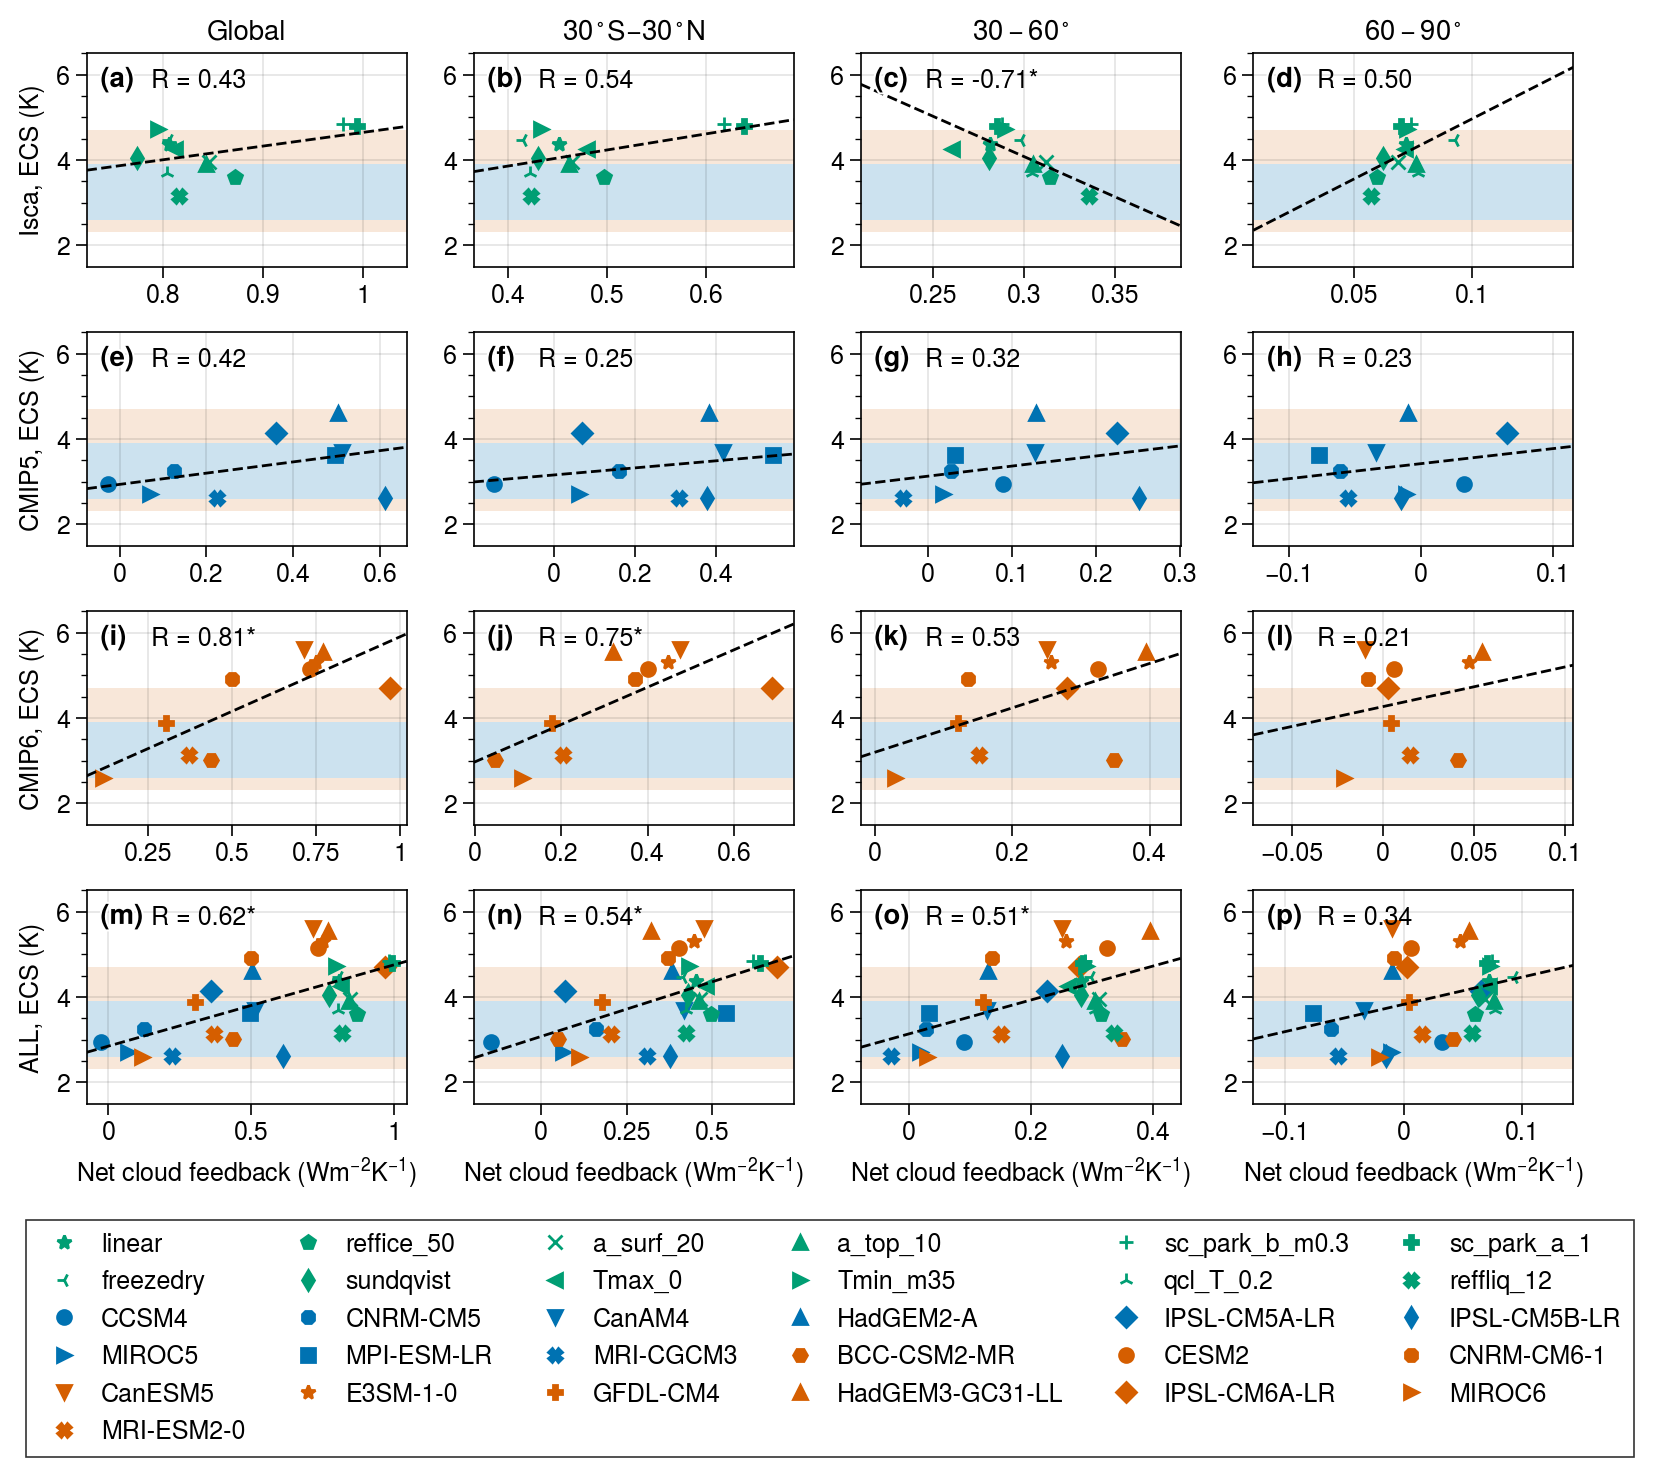
\includegraphics[width=0.9\linewidth]{{figs/change_of_CRE/ECS_vs_cldfbk_all_ALL_cmip56_isca}.png}
    \caption{The scatter plot of equilibrium climate sensitivity (ECS; K) against the net cloud feedbacks (Wm$^{-2}$K$^{-1}$) from different models and different regions. Rows from top to bottom are for Isca (green), CMIP5 (blue), CMIP6 (orange) models and all of them, respectively. From left to right, the columns are for global, tropical (30$^\circ$S--30$^\circ$N), midlatitude (30-60$^\circ$), and high latitude (60-90$^\circ$) regions, respectively. The blue shaded indicates the 17th and 83rd percentile range of the Baseline probability density function of ECS from \cite{Sherwood2020}, while the orange shaded indicates the 5th to 95th percentile range. The dashed lines are liner regression of ECS against cloud feedbacks, and the the correlation coefficient ($R$) with asterisk is above 95\% confidence interval.}
    \label{fig:ECS_vs_cld_fbk_from_diff_regions}
\end{figure}

\begin{figure}[ht]
    \centering
    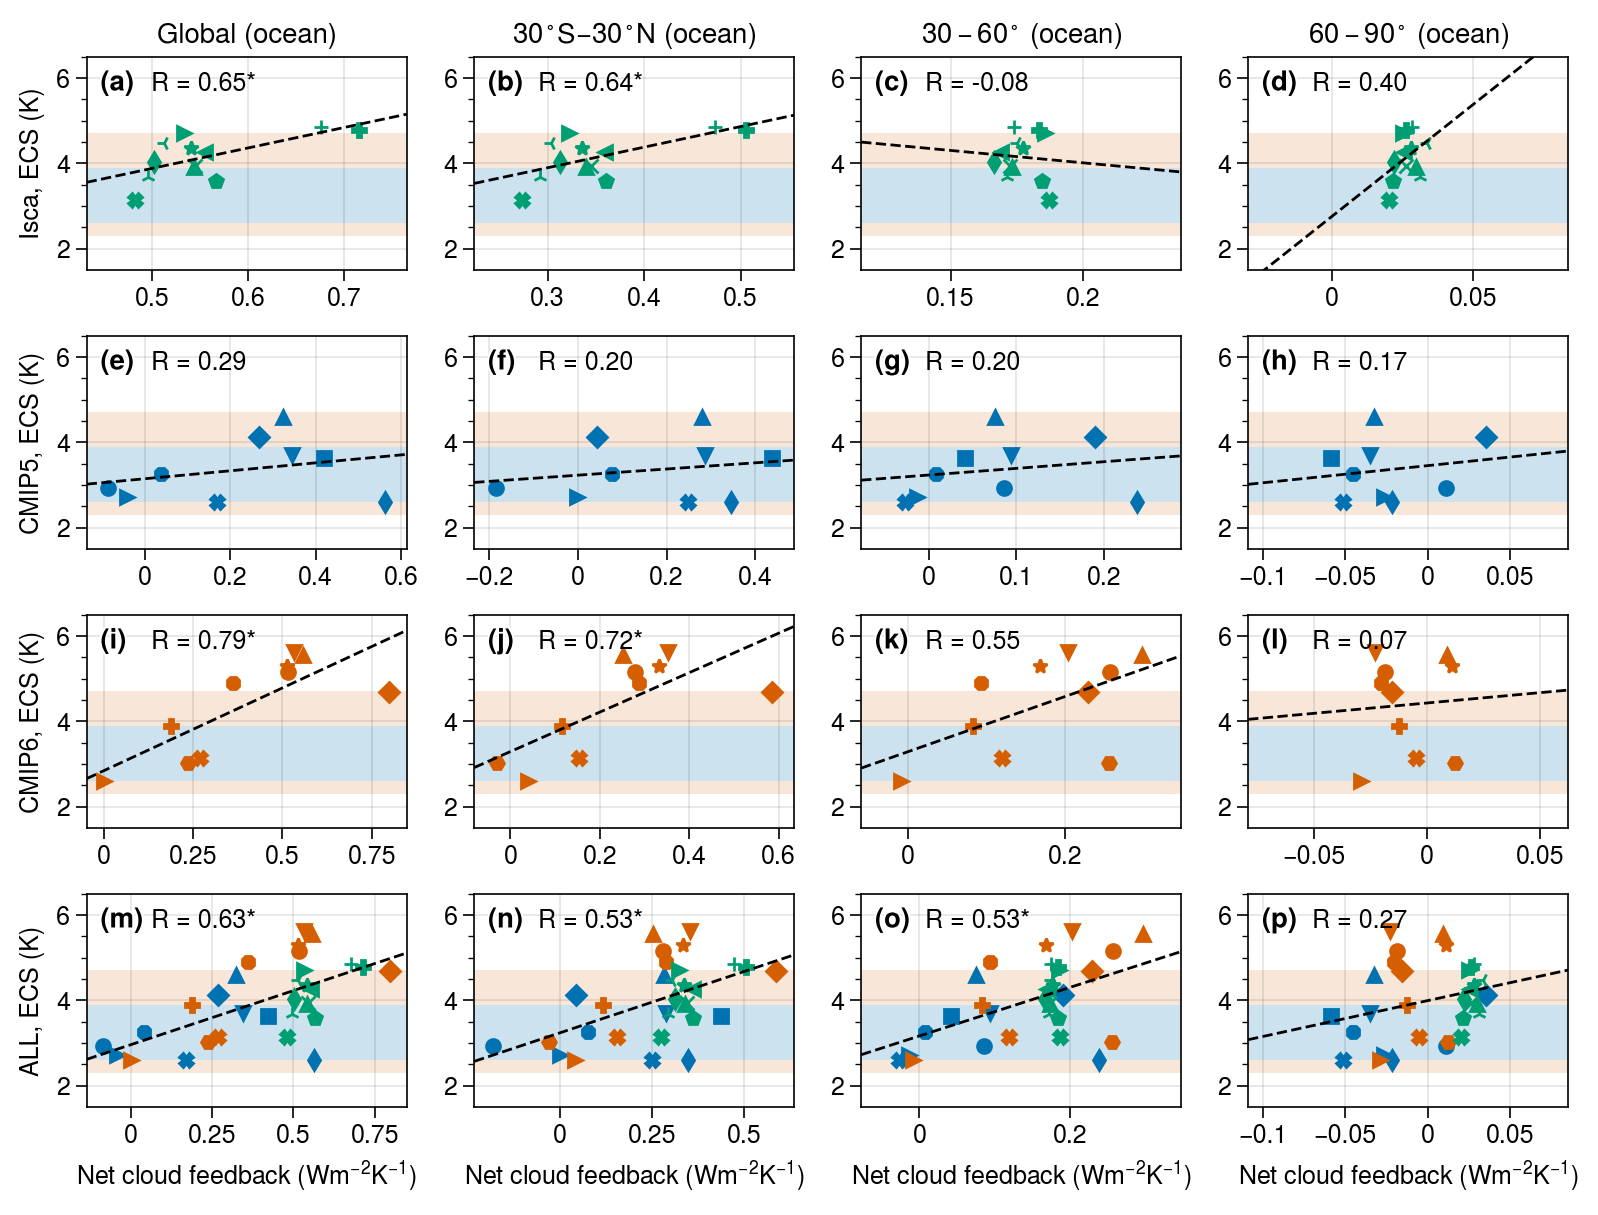
\includegraphics[width=0.9\linewidth]{{figs/change_of_CRE/ECS_vs_cldfbk_ocean_ALL_cmip56_isca_no_legend}.png}
    \caption{As in \figref{fig:ECS_vs_cld_fbk_from_diff_regions}, but for cloud feedbacks from ocean regions only. Symbols are the same as \figref{fig:ECS_vs_cld_fbk_from_diff_regions}.}
    \label{fig:ECS_vs_cld_fbk_from_diff_ocn_regions}
\end{figure}

As both feedbacks and ECS display certain range (\tabref{tab:ECS_forcing_feedback}), is there any relationship between the spread in ECS and the spread in cloud feedbacks in Isca PPE simulations? Previous studies have confirmed that the cloud feedback uncertainty is the largest source of intermodel spread of ECS in CMIP models \cite[e.g.,][]{Ceppi2017,Zelinka2020causes}. In addition, \cite{Zelinka2020causes} find the inter-model spread of ECS in CMIP5/6 models is well related the spread of global mean cloud feedbacks (see their Fig. S4). However, this linear relationship may not be robust across all the regions or across models with different ECS \citep{Lutsko2021emergent}. Therefore, here we check the relationship between the spread of ECS and cloud feedback in Isca PPE simulations. As shown in \figref{fig:ECS_vs_cld_fbk_from_diff_regions}, the ECS of Isca PPE did not show a robust linear relationship against cloud feedback for global and tropical (30$^\circ$S--30$^\circ$N) and high latitude (60$^\circ$S--90$^\circ$) regions (first row). The anticorrelation of ECS and cloud feedback in midlatitude region (30$^\circ$S--60$^\circ$) of Isca (\figref{fig:ECS_vs_cld_fbk_from_diff_regions}c) could be fortuitous or artifacts of the PPE, as the perturbations are limited to a very narrow range. Another reason saying so is because we find the Isca PPE does display a relative narrow scope at the midlatitude when combining with part of CMIP5/6 models (\figref{fig:ECS_vs_cld_fbk_from_diff_regions}o). We also find such linear relationships are not robust among CMIP5 models both for global and different regions (\figsref{fig:ECS_vs_cld_fbk_from_diff_regions}e--h), but it is robust for global in CMIP5 \citep[see their Fig. S4 in][]{Zelinka2020causes}. The discrepancy is perhaps due to the fact that only the 9 CMIP5 models that are implemented with the COSP are used in this research \citep{Zelinka2021evaluating}, while almost all the models are employed in \cite{Zelinka2020causes}. With regard to CMIP6 models, it is the same that only the ones implemented with COSP are selected, but they still show robust linear relationship between ECS and cloud feedback both for global and tropical regions (\figsref{fig:ECS_vs_cld_fbk_from_diff_regions}i and j). Nevertheless, when all the Isca and CMIP models are used for the regression, the ECS and cloud feedbacks are linear correlated with each other for global, tropical and midlatitude regions (last row of \figref{fig:ECS_vs_cld_fbk_from_diff_regions}).

\begin{figure}[ht]
    \centering
    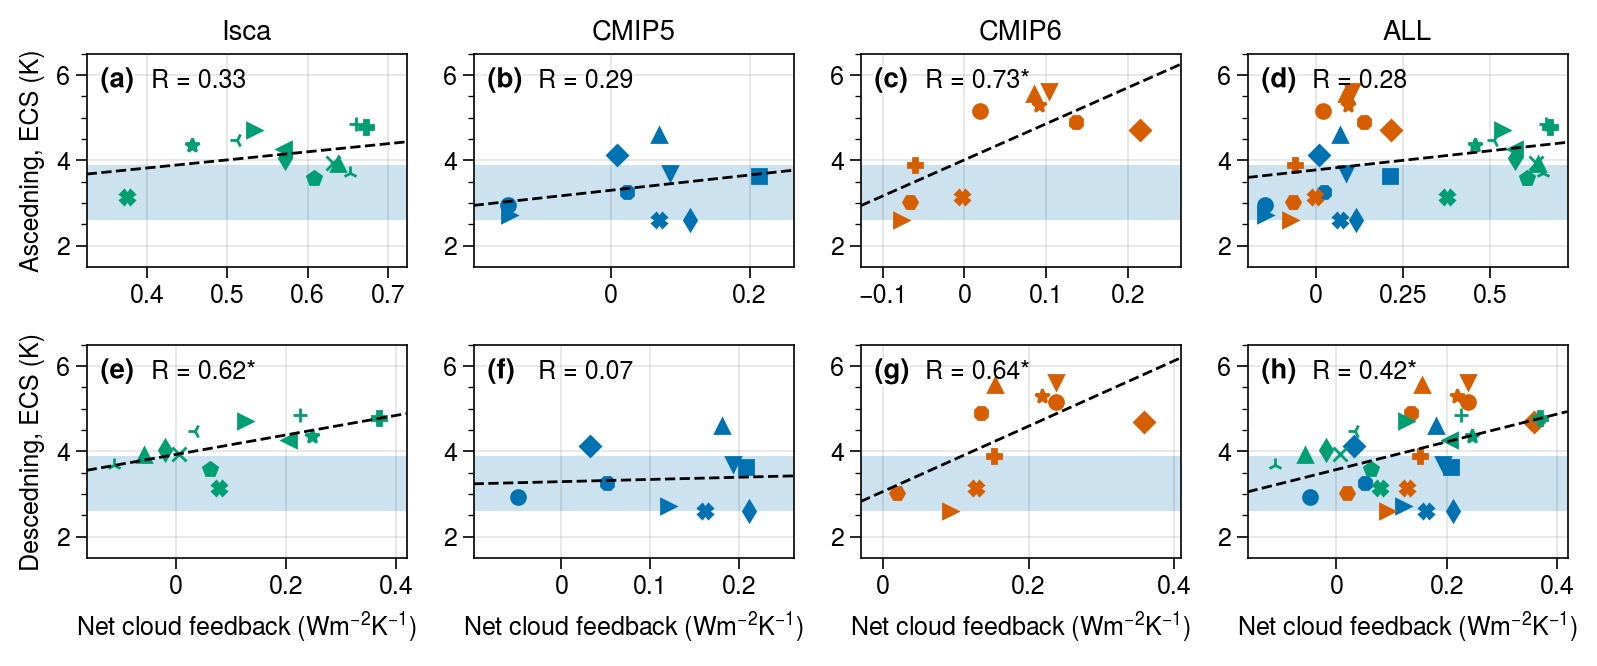
\includegraphics[width=1\linewidth]{{figs/change_of_CRE/ECS_vs_cldfbk_ALL_cmip56_isca_tropical_asc_dsc_no_legend}.png}
    \caption{As in \figref{fig:ECS_vs_cld_fbk_from_diff_regions}, but for cloud feedbacks from tropical (top) ascending and (bottom) descending regions respectively, and the regimes are decomposed based on vertical velocity at 500 hPa. Symbols keep the same as \figref{fig:ECS_vs_cld_fbk_from_diff_regions}.}
    \label{fig:ECS_vs_cld_fbk_from_diff_ocn_asc_dsc_regions}
\end{figure}

Similarly, when the analysis is repeated for ocean region only, we find that the linear relationship is robust in global and tropical regions for Isca, CMIP6 and when all the models are used, but not robust for CMIP5 models (\figref{fig:ECS_vs_cld_fbk_from_diff_ocn_regions}). It is noted that this relationship is not robust for Isca when both land and ocean are involved (first row of \figref{fig:ECS_vs_cld_fbk_from_diff_regions}), indicating that the cloud feedbacks from ocean regions, especially tropical oceans, are more relevant to the spread of ECS. Inspired by this, after decomposing the tropical ocean region into ascending and descending regimes according to vertical velocity at 500 hPa \citep{Bony2004,Bony2005} and reiterating the analysis, we find the linear relationship of ECS and cloud feedback is only robust in descending regime for Isca simulations (\figsref{fig:ECS_vs_cld_fbk_from_diff_ocn_asc_dsc_regions}a and e). Also considering the whole tropical ocean region shows a robust correlation in \figref{fig:ECS_vs_cld_fbk_from_diff_ocn_regions}b, this implies that the cloud feedback in subsidence regime is key to understand the spread of ECS in Isca, consistent with the conclusions in \secref{sec:reg_contri_to_spread_of_cldfbk}. The CMIP5 models used in this study did not show robust linear relationship for both dynamical regimes, while CMIP6 models show robust results for both regimes. When all the models are involved for the regression, the linear relationship is only robust in descending regime, reflecting that low cloud feedback in subsidence regime play an important role in determining the spread of total cloud feedback (\secref{sec:reg_contri_to_spread_of_cldfbk}) and ECS.


\section{Summary and discussion}

Cloud feedback has the largest intermodel spread among all the feedback parameters in CMIP5/6 models \citep{Zelinka2020causes}, one of the largest sources of uncertainty in ECS among GCMs \citep{Stocker2013,Ceppi2017,Zelinka2020causes}, but the underlying causes for cloud feedback uncertainty are still not fully understood \citep[e.g.,][]{Bony2005,Vial2013,Qu2014,Qu2015positive,Webb2015,Zelinka2016insights,Geoffroy2017,Zelinka2020causes}. Narrowing down the cloud feedback uncertainty is key to constrain the range of ECS \citep[e.g.,][]{Myers2021,Ceppi2021observational} and to help us better understand the responses of climate system to global warming. In this chapter, we try to use the simple cloud scheme developed in \chapref{ch:simple_cld_scheme} to understand the spread of cloud feedbacks. 

At first, we try to evaluate the simulated cloud feedback from the simple diagnostic cloud scheme (described in \chapref{ch:simple_cld_scheme}) of Isca. To do so, the CFMIP observation simulator pacakage (COSP) is implemented in Isca to get the necessary outputs to be used for the cloud feedback calculation and decomposition. The COSP output was evaluated first to make sure it is successfully implemented. Then,  the cloud radiative kernel method \citep{Zelinka2012computing1,Zelinka2012computing2} is employed

At first, the simulated cloud feedbacks, including their spatial pattern and zonal mean structure, as well as their various components, are evaluated. Then the spread of cloud feedbacks in Isca PPE and the possible underlying causes 


With the implemented in Isca, the cloud feedback cloud radiative kernel method,

Conclusions

To do next?